% REFERENCE COPY, made on 11 Oct 2026 at Alexandru's request: the documentation as it was before the
% shortening to 8 pages began (sha bc856e97, 15 pages, body ending on page 12). Kept for comparison only;
% the working file is documentatie_overleaf.tex. Only change below this block: the author placeholder removed
% (11 Oct 2026, asked by Alexandru).

% =====================================================================
% Course documentation on the full official ACL template (acl_latex.tex,
% acl-org/acl-style-files, also used by NAACL), option `final`.
% Method: release/ (anonymous repo). Numbers: release/fuse.py, saved in
%   output/doc_fuse_ro11.*    11 languages, main result
%   output/doc_fuse_mlsp10.*  10 MLSP languages, separate run
% Each number has its source in a comment next to it.
% Overleaf: project from the ACL template, paste this file over
% acl_latex.tex, upload figures/. custom.bib is rewritten by the block below.
% =====================================================================

\begin{filecontents*}[overwrite]{custom.bib}
@inproceedings{yimam-etal-2018-report,
    title = "A Report on the Complex Word Identification Shared Task 2018",
    author = {Yimam, Seid Muhie  and
      Biemann, Chris  and
      Malmasi, Shervin  and
      Paetzold, Gustavo  and
      Specia, Lucia  and
      {\v{S}}tajner, Sanja  and
      Tack, Ana{\"i}s  and
      Zampieri, Marcos},
    booktitle = "Proceedings of the Thirteenth Workshop on Innovative Use of {NLP} for Building Educational Applications",
    month = jun,
    year = "2018",
    address = "New Orleans, Louisiana",
    publisher = "Association for Computational Linguistics",
    url = "https://aclanthology.org/W18-0507/",
    doi = "10.18653/v1/W18-0507",
    pages = "66--78"
}

@inproceedings{shardlow-etal-2021-semeval,
    title = "{S}em{E}val-2021 Task 1: Lexical Complexity Prediction",
    author = "Shardlow, Matthew  and
      Evans, Richard  and
      Paetzold, Gustavo Henrique  and
      Zampieri, Marcos",
    booktitle = "Proceedings of the 15th International Workshop on Semantic Evaluation (SemEval-2021)",
    month = aug,
    year = "2021",
    address = "Online",
    publisher = "Association for Computational Linguistics",
    url = "https://aclanthology.org/2021.semeval-1.1/",
    doi = "10.18653/v1/2021.semeval-1.1",
    pages = "1--16"
}

@inproceedings{shardlow-etal-2024-multilingual,
    title = "Multilingual Resources for Lexical Complexity Prediction: A Review",
    author = "Shardlow, Matthew  and
      North, Kai  and
      Zampieri, Marcos",
    booktitle = "Proceedings of the Workshop on DeTermIt! Evaluating Text Difficulty in a Multilingual Context @ LREC-COLING 2024",
    month = may,
    year = "2024",
    address = "Torino, Italia",
    publisher = "ELRA and ICCL",
    url = "https://aclanthology.org/2024.determit-1.5/",
    pages = "51--59"
}

@inproceedings{shardlow-etal-2024-bea,
    title = "The {BEA} 2024 Shared Task on the Multilingual Lexical Simplification Pipeline",
    author = {Shardlow, Matthew  and
      Alva-Manchego, Fernando  and
      Batista-Navarro, Riza  and
      Bott, Stefan  and
      Calderon Ramirez, Saul  and
      Cardon, R{\'e}mi  and
      Fran{\c{c}}ois, Thomas  and
      Hayakawa, Akio  and
      Horbach, Andrea  and
      H{\"u}lsing, Anna  and
      Ide, Yusuke  and
      Imperial, Joseph Marvin  and
      Nohejl, Adam  and
      North, Kai  and
      Occhipinti, Laura  and
      Rojas, Nelson Per{\'e}z  and
      Raihan, Nishat  and
      Ranasinghe, Tharindu  and
      Salazar, Martin Solis  and
      {\v{S}}tajner, Sanja  and
      Zampieri, Marcos  and
      Saggion, Horacio},
    booktitle = "Proceedings of the 19th Workshop on Innovative Use of NLP for Building Educational Applications (BEA 2024)",
    month = jun,
    year = "2024",
    address = "Mexico City, Mexico",
    publisher = "Association for Computational Linguistics",
    url = "https://aclanthology.org/2024.bea-1.51/",
    pages = "571--589"
}

@inproceedings{saggion-etal-2024-lexical,
    title = "Lexical Complexity Prediction and Lexical Simplification for {C}atalan and {S}panish: Resource Creation, Quality Assessment, and Ethical Considerations",
    author = "Saggion, Horacio  and
      Bott, Stefan  and
      Szasz, Sandra  and
      P{\'e}rez, Nelson  and
      Calder{\'o}n, Sa{\'u}l  and
      Sol{\'i}s, Mart{\'i}n",
    booktitle = "Proceedings of the Third Workshop on Text Simplification, Accessibility and Readability (TSAR 2024)",
    month = nov,
    year = "2024",
    address = "Miami, Florida, USA",
    publisher = "Association for Computational Linguistics",
    url = "https://aclanthology.org/2024.tsar-1.9/",
    doi = "10.18653/v1/2024.tsar-1.9",
    pages = "82--94"
}

@inproceedings{qiu-etal-2024-complex,
    title = "{C}omp{L}ex-{ZH}: A New Dataset for Lexical Complexity Prediction in {M}andarin and {C}antonese",
    author = "Qiu, Le  and
      Guo, Shanyue  and
      Wong, Tak-Sum  and
      Chersoni, Emmanuele  and
      Lee, John  and
      Huang, Chu-Ren",
    booktitle = "Proceedings of the Third Workshop on Text Simplification, Accessibility and Readability (TSAR 2024)",
    month = nov,
    year = "2024",
    address = "Miami, Florida, USA",
    publisher = "Association for Computational Linguistics",
    url = "https://aclanthology.org/2024.tsar-1.3/",
    doi = "10.18653/v1/2024.tsar-1.3",
    pages = "20--26"
}

@inproceedings{anghel-etal-2025-rals,
    title = "{RALS}: Resources and Baselines for {R}omanian Automatic Lexical Simplification",
    author = "Anghel, Fabian  and
      Cristea, Petru Theodor  and
      Creang{\u{a}}, Claudiu  and
      Nisioi, Sergiu",
    booktitle = "Proceedings of the 2025 Conference on Empirical Methods in Natural Language Processing",
    month = nov,
    year = "2025",
    address = "Suzhou, China",
    publisher = "Association for Computational Linguistics",
    url = "https://aclanthology.org/2025.emnlp-main.1603/",
    doi = "10.18653/v1/2025.emnlp-main.1603",
    pages = "31481--31492"
}

@inproceedings{cristea-nisioi-2024-machine,
    title = "Archaeology at {MLSP} 2024: Machine Translation for Lexical Complexity Prediction and Lexical Simplification",
    author = "Cristea, Petru  and
      Nisioi, Sergiu",
    booktitle = "Proceedings of the 19th Workshop on Innovative Use of NLP for Building Educational Applications (BEA 2024)",
    month = jun,
    year = "2024",
    address = "Mexico City, Mexico",
    publisher = "Association for Computational Linguistics",
    url = "https://aclanthology.org/2024.bea-1.55/",
    pages = "610--617"
}

@inproceedings{enomoto-etal-2024-tmu,
    title = "{TMU}-{HIT} at {MLSP} 2024: How Well Can {GPT}-4 Tackle Multilingual Lexical Simplification?",
    author = "Enomoto, Taisei  and
      Kim, Hwichan  and
      Hirasawa, Tosho  and
      Nagai, Yoshinari  and
      Sato, Ayako  and
      Nakajima, Kyotaro  and
      Komachi, Mamoru",
    booktitle = "Proceedings of the 19th Workshop on Innovative Use of NLP for Building Educational Applications (BEA 2024)",
    month = jun,
    year = "2024",
    address = "Mexico City, Mexico",
    publisher = "Association for Computational Linguistics",
    url = "https://aclanthology.org/2024.bea-1.52/",
    pages = "590--598"
}

@article{nohejl-etal-2025-japanese,
    author  = {Nohejl, Adam and Hayakawa, Akio and Ide, Yusuke and Watanabe, Taro},
    title   = {A {J}apanese Dataset and Efficient Multilingual {LLM}-Based Methods for Lexical Simplification and Lexical Complexity Prediction},
    journal = {Journal of Natural Language Processing},
    volume  = {32},
    number  = {4},
    pages   = {1129--1188},
    year    = {2025},
    doi     = {10.5715/jnlp.32.1129}
}

@inproceedings{liu-etal-2023-geval,
    title     = "{G}-{E}val: {NLG} Evaluation using {GPT}-4 with Better Human Alignment",
    author    = "Liu, Yang  and
      Iter, Dan  and
      Xu, Yichong  and
      Wang, Shuohang  and
      Xu, Ruochen  and
      Zhu, Chenguang",
    booktitle = "Proceedings of the 2023 Conference on Empirical Methods in Natural Language Processing",
    month     = dec,
    year      = "2023",
    address   = "Singapore",
    publisher = "Association for Computational Linguistics",
    url       = "https://aclanthology.org/2023.emnlp-main.153/",
    doi       = "10.18653/v1/2023.emnlp-main.153",
    pages     = "2511--2522"
}

@inproceedings{conneau2020xlmr,
    title     = "Unsupervised Cross-lingual Representation Learning at Scale",
    author    = "Conneau, Alexis  and
      Khandelwal, Kartikay  and
      Goyal, Naman  and
      Chaudhary, Vishrav  and
      Wenzek, Guillaume  and
      Guzm{\'a}n, Francisco  and
      Grave, Edouard  and
      Ott, Myle  and
      Zettlemoyer, Luke  and
      Stoyanov, Veselin",
    booktitle = "Proceedings of the 58th Annual Meeting of the Association for Computational Linguistics",
    month     = jul,
    year      = "2020",
    address   = "Online",
    publisher = "Association for Computational Linguistics",
    url       = "https://aclanthology.org/2020.acl-main.747/",
    doi       = "10.18653/v1/2020.acl-main.747",
    pages     = "8440--8451"
}

@inproceedings{pires-etal-2019-multilingual,
    title = "How Multilingual is Multilingual {BERT}?",
    author = "Pires, Telmo  and
      Schlinger, Eva  and
      Garrette, Dan",
    booktitle = "Proceedings of the 57th Annual Meeting of the Association for Computational Linguistics",
    month = jul,
    year = "2019",
    address = "Florence, Italy",
    publisher = "Association for Computational Linguistics",
    url = "https://aclanthology.org/P19-1493/",
    doi = "10.18653/v1/P19-1493",
    pages = "4996--5001"
}

@inproceedings{wu-dredze-2020-languages,
    title = "Are All Languages Created Equal in Multilingual {BERT}?",
    author = "Wu, Shijie  and
      Dredze, Mark",
    booktitle = "Proceedings of the 5th Workshop on Representation Learning for NLP",
    month = jul,
    year = "2020",
    address = "Online",
    publisher = "Association for Computational Linguistics",
    url = "https://aclanthology.org/2020.repl4nlp-1.16/",
    doi = "10.18653/v1/2020.repl4nlp-1.16",
    pages = "120--130"
}

% checked on aclanthology.org/2021.repl4nlp-1.8 (title, four authors, RepL4NLP 2021, pages 64--71, DOI), 11 Oct 2026.
@inproceedings{liu-etal-2021-preserving,
    title = "Preserving Cross-Linguality of Pre-trained Models via Continual Learning",
    author = "Liu, Zihan  and
      Winata, Genta Indra  and
      Madotto, Andrea  and
      Fung, Pascale",
    booktitle = "Proceedings of the 6th Workshop on Representation Learning for NLP (RepL4NLP-2021)",
    month = aug,
    year = "2021",
    address = "Online",
    publisher = "Association for Computational Linguistics",
    url = "https://aclanthology.org/2021.repl4nlp-1.8/",
    doi = "10.18653/v1/2021.repl4nlp-1.8",
    pages = "64--71"
}

@inproceedings{peters-etal-2019-tune,
    title = "To Tune or Not to Tune? Adapting Pretrained Representations to Diverse Tasks",
    author = "Peters, Matthew E.  and
      Ruder, Sebastian  and
      Smith, Noah A.",
    booktitle = "Proceedings of the 4th Workshop on Representation Learning for NLP (RepL4NLP-2019)",
    month = aug,
    year = "2019",
    address = "Florence, Italy",
    publisher = "Association for Computational Linguistics",
    url = "https://aclanthology.org/W19-4302/",
    doi = "10.18653/v1/W19-4302",
    pages = "7--14"
}

@inproceedings{feng-etal-2022-language,
    title     = "Language-agnostic {BERT} Sentence Embedding",
    author    = "Feng, Fangxiaoyu  and
      Yang, Yinfei  and
      Cer, Daniel  and
      Arivazhagan, Naveen  and
      Wang, Wei",
    booktitle = "Proceedings of the 60th Annual Meeting of the Association for Computational Linguistics (Volume 1: Long Papers)",
    month     = may,
    year      = "2022",
    address   = "Dublin, Ireland",
    publisher = "Association for Computational Linguistics",
    url       = "https://aclanthology.org/2022.acl-long.62/",
    doi       = "10.18653/v1/2022.acl-long.62",
    pages     = "878--891"
}

@article{wang2024multilinguale5,
    author  = {Wang, Liang and Yang, Nan and Huang, Xiaolong and Yang, Linjun and Majumder, Rangan and Wei, Furu},
    title   = {Multilingual {E}5 Text Embeddings: A Technical Report},
    journal = {Computing Research Repository},
    volume  = {arXiv:2402.05672},
    year    = {2024},
    url     = {https://arxiv.org/abs/2402.05672}
}

@inproceedings{libovicky-etal-2020-language,
    title = "On the Language Neutrality of Pre-trained Multilingual Representations",
    author = "Libovick{\'y}, Jind{\v{r}}ich  and
      Rosa, Rudolf  and
      Fraser, Alexander",
    booktitle = "Findings of the Association for Computational Linguistics: {EMNLP} 2020",
    month = nov,
    year = "2020",
    address = "Online",
    publisher = "Association for Computational Linguistics",
    url = "https://aclanthology.org/2020.findings-emnlp.150/",
    doi = "10.18653/v1/2020.findings-emnlp.150",
    pages = "1663--1674"
}

@inproceedings{qi-etal-2020-stanza,
    title     = "{S}tanza: A {P}ython Natural Language Processing Toolkit for Many Human Languages",
    author    = "Qi, Peng  and
      Zhang, Yuhao  and
      Zhang, Yuhui  and
      Bolton, Jason  and
      Manning, Christopher D.",
    booktitle = "Proceedings of the 58th Annual Meeting of the Association for Computational Linguistics: System Demonstrations",
    month     = jul,
    year      = "2020",
    address   = "Online",
    publisher = "Association for Computational Linguistics",
    url       = "https://aclanthology.org/2020.acl-demos.14/",
    doi       = "10.18653/v1/2020.acl-demos.14",
    pages     = "101--108"
}

@inproceedings{rust-etal-2021-good,
    title     = "How Good is Your Tokenizer? On the Monolingual Performance of Multilingual Language Models",
    author    = "Rust, Phillip  and
      Pfeiffer, Jonas  and
      Vuli{\'c}, Ivan  and
      Ruder, Sebastian  and
      Gurevych, Iryna",
    booktitle = "Proceedings of the 59th Annual Meeting of the Association for Computational Linguistics and the 11th International Joint Conference on Natural Language Processing (Volume 1: Long Papers)",
    month     = aug,
    year      = "2021",
    address   = "Online",
    publisher = "Association for Computational Linguistics",
    url       = "https://aclanthology.org/2021.acl-long.243/",
    doi       = "10.18653/v1/2021.acl-long.243",
    pages     = "3118--3135"
}

@inproceedings{gorman-bedrick-2019-need,
    title = "We Need to Talk about Standard Splits",
    author = "Gorman, Kyle  and
      Bedrick, Steven",
    booktitle = "Proceedings of the 57th Annual Meeting of the Association for Computational Linguistics",
    month = jul,
    year = "2019",
    address = "Florence, Italy",
    publisher = "Association for Computational Linguistics",
    url = "https://aclanthology.org/P19-1267/",
    doi = "10.18653/v1/P19-1267",
    pages = "2786--2791"
}

@inproceedings{lundberg-lee-2017-unified,
    title     = {A Unified Approach to Interpreting Model Predictions},
    author    = {Lundberg, Scott M. and Lee, Su-In},
    booktitle = {Advances in Neural Information Processing Systems 30},
    pages     = {4765--4774},
    year      = {2017},
    url       = {https://papers.nips.cc/paper/7062-a}
}

@article{lundberg-etal-2020-trees,
    title   = {From Local Explanations to Global Understanding with Explainable {AI} for Trees},
    author  = {Lundberg, Scott M. and Erion, Gabriel and Chen, Hugh and DeGrave, Alex and
               Prutkin, Jordan M. and Nair, Bala and Katz, Ronit and Himmelfarb, Jonathan and
               Bansal, Nisha and Lee, Su-In},
    journal = {Nature Machine Intelligence},
    volume  = {2},
    number  = {1},
    pages   = {56--67},
    year    = {2020},
    doi     = {10.1038/s42256-019-0138-9}
}

% arXiv:2607.02770, checked on export.arxiv.org (title, corporate author, 2026).
@article{gemmateam-2026-gemma4,
    author  = {{Gemma Team}},
    title   = {Gemma 4 Technical Report},
    journal = {Computing Research Repository},
    volume  = {arXiv:2607.02770},
    year    = {2026},
    url     = {https://arxiv.org/abs/2607.02770}
}

% arXiv:2505.09388, checked on export.arxiv.org (60 authors, first An Yang).
@article{yang-etal-2025-qwen3,
    author  = {Yang, An and Li, Anfeng and Yang, Baosong and Zhang, Beichen and Hui, Binyuan and Zheng, Bo and others},
    title   = {{Qwen3} Technical Report},
    journal = {Computing Research Repository},
    volume  = {arXiv:2505.09388},
    year    = {2025},
    url     = {https://arxiv.org/abs/2505.09388}
}

% Zenodo, DOI 10.5281/zenodo.7199437, checked on zenodo.org (Robyn Speer, 2022).
@misc{speer-2022-wordfreq,
    author    = {Speer, Robyn},
    title     = {rspeer/wordfreq: v3.0},
    year      = {2022},
    publisher = {Zenodo},
    doi       = {10.5281/zenodo.7199437}
}

@article{vandermaaten-hinton-2008-tsne,
    title   = {Visualizing Data using t-{SNE}},
    author  = {van der Maaten, Laurens and Hinton, Geoffrey},
    journal = {Journal of Machine Learning Research},
    volume  = {9},
    pages   = {2579--2605},
    year    = {2008}
}

% DOI 10.1145/3715669.3726843, checked on Crossref on 11 Oct 2026 (75 authors, first Deborah N. Jakobi).
@inproceedings{jakobi-etal-2025-multipleye,
    author    = {Jakobi, Deborah Noemie and Stegenwallner-Sch{\"u}tz, Maja and Hollenstein, Nora and Ding, Cui and Kaspere, Ramune and others},
    title     = {{MultiplEYE}: Creating a Multilingual Eye-Tracking-While-Reading Corpus},
    booktitle = {Proceedings of the 2025 Symposium on Eye Tracking Research and Applications},
    series    = {ETRA '25},
    publisher = {ACM},
    year      = {2025},
    pages     = {1--11},
    doi       = {10.1145/3715669.3726843}
}
\end{filecontents*}

\documentclass[11pt]{article}

% Change "review" to "final" to generate the final (sometimes called camera-ready) version.
% Change to "preprint" to generate a non-anonymous version with page numbers.
\usepackage[final]{acl}

% Standard package includes
\usepackage{times}
\usepackage{latexsym}

% For proper rendering and hyphenation of words containing Latin characters (including in bib files)
\usepackage[T1]{fontenc}
% For Vietnamese characters
% \usepackage[T5]{fontenc}
% See https://www.latex-project.org/help/documentation/encguide.pdf for other character sets

% This assumes your files are encoded as UTF8
\usepackage[utf8]{inputenc}

% This is not strictly necessary, and may be commented out,
% but it will improve the layout of the manuscript,
% and will typically save some space.
\usepackage{microtype}

% This is also not strictly necessary, and may be commented out.
% However, it will improve the aesthetics of text in
% the typewriter font.
\usepackage{inconsolata}

%Including images in your LaTeX document requires adding
%additional package(s)
\usepackage{graphicx}

% If the title and author information does not fit in the area allocated, uncomment the following
%
%\setlength\titlebox{<dim>}
%
% and set <dim> to something 5cm or larger.

% Added on top of the template.
\usepackage{booktabs}          % \toprule / \midrule / \bottomrule in the tables
\graphicspath{{figures/}}

% The default fractions (topfraction 0.7, textfraction 0.2) give whole columns
% to tables; relaxed so that text fits next to a float.
\renewcommand{\topfraction}{0.9}
\renewcommand{\bottomfraction}{0.5}
\renewcommand{\textfraction}{0.08}
\renewcommand{\floatpagefraction}{0.8}

\title{Lexical Complexity Prediction Without Target-Language Labels}

% Author information can be set in various styles:
% For several authors from the same institution:
% \author{Author 1 \and ... \and Author n \\
%         Address line \\ ... \\ Address line}
% if the names do not fit well on one line use
%         Author 1 \\ {\bf Author 2} \\ ... \\ {\bf Author n} \\
% For authors from different institutions:
% \author{Author 1 \\ Address line \\  ... \\ Address line
%         \And  ... \And
%         Author n \\ Address line \\ ... \\ Address line}
% To start a separate ``row'' of authors use \AND, as in
% \author{Author 1 \\ Address line \\  ... \\ Address line
%         \AND
%         Author 2 \\ Address line \\ ... \\ Address line \And
%         Author 3 \\ Address line \\ ... \\ Address line}

% Authors removed on 11 Oct 2026 at Alexandru's request (the ARR submission is anonymous), as in documentatie_overleaf.tex.
\author{}

%\author{
%  \textbf{First Author\textsuperscript{1}},
%  \textbf{Second Author\textsuperscript{1,2}},
%  \textbf{Third T. Author\textsuperscript{1}},
%  \textbf{Fourth Author\textsuperscript{1}},
%\\
%  \textbf{Fifth Author\textsuperscript{1,2}},
%  \textbf{Sixth Author\textsuperscript{1}},
%  \textbf{Seventh Author\textsuperscript{1}},
%  \textbf{Eighth Author \textsuperscript{1,2,3,4}},
%\\
%  \textbf{Ninth Author\textsuperscript{1}},
%  \textbf{Tenth Author\textsuperscript{1}},
%  \textbf{Eleventh E. Author\textsuperscript{1,2,3,4,5}},
%  \textbf{Twelfth Author\textsuperscript{1}},
%\\
%  \textbf{Thirteenth Author\textsuperscript{3}},
%  \textbf{Fourteenth F. Author\textsuperscript{2,4}},
%  \textbf{Fifteenth Author\textsuperscript{1}},
%  \textbf{Sixteenth Author\textsuperscript{1}},
%\\
%  \textbf{Seventeenth S. Author\textsuperscript{4,5}},
%  \textbf{Eighteenth Author\textsuperscript{3,4}},
%  \textbf{Nineteenth N. Author\textsuperscript{2,5}},
%  \textbf{Twentieth Author\textsuperscript{1}}
%\\
%\\
%  \textsuperscript{1}Affiliation 1,
%  \textsuperscript{2}Affiliation 2,
%  \textsuperscript{3}Affiliation 3,
%  \textsuperscript{4}Affiliation 4,
%  \textsuperscript{5}Affiliation 5
%\\
%  \small{
%    \textbf{Correspondence:} \href{mailto:email@domain}{email@domain}
%  }
%}

\begin{document}
\maketitle

% Keywords before the abstract, as in the glioma paper, with the abstract's margins.
% Revised on 11 Oct 2026, asked by Alexandru: Zero-Label Evaluation dropped (it named the protocol,
% already covered by Leave-One-Language-Out), Eye-Tracking added (Section 5).
\begin{list}{}{\setlength{\rightmargin}{0.6cm}\setlength{\leftmargin}{0.6cm}}
\item[] \textbf{Keywords:} Lexical Complexity Prediction, Cross-Lingual Transfer,
Leave-One-Language-Out, Multilingual Encoders, Large Language Models, Eye-Tracking
\end{list}

\begin{abstract}
% Text by Gemma 4 12B (mlx-community/gemma-4-12B-it-qat-OptiQ-4bit, revision 63912b88), asked by
% Alexandru on 11 Oct 2026: a rewrite of our draft, approved in chat, with docs/PROMPT_gemma_abstract.txt
% and docs/gemma_introducere.py (temperature 0.7, top-p 0.95, seed 0, thinking off). Then four revisions
% asked by Alexandru, each from the previous answer: _v2 ("test language"; the 30 labels are of each
% evaluated language), _v3 (first sentence dropped, the model not named, all the languages of the
% evaluation data), _v4 (his wording for the two regressors and the zero-shot prompt), _v5 ("setting
% selection" dropped). Inserted unchanged.
We predict word complexity in a test language using only labelled data from other languages. Our
method fuses two signals via a weighted average. The first signal combines two regressor models,
ridge regression and gradient-boosted trees, trained on word features and embeddings from three
frozen multilingual encoders. The second signal is the expected rating of an open-weight LLM, using % Gemma 4 12B, chosen on the other languages for all eleven test languages (doc_fuse_ro11.txt, column model)
zero-shot prompt without fine-tuning. We use no labels from the test language for training. We % release/signal_a.py:146-147: CompLex is left out when English is the test language
evaluate our approach using a leave-one-language-out protocol on all the languages of the evaluation
data. Over these eleven languages, the mean Pearson correlation is 0.693, with a 95\% interval of % doc_fuse_ro11.txt, mean line: 0.692521 [0.6789, 0.7057]
0.679 to 0.706. The mean on the ten MLSP 2024 languages is 0.690. The highest published mean on MLSP % doc_fuse_mlsp10.txt, mean line: 0.689745
2024 is 0.669, achieved by a method that reads 30 labels of each evaluated language. % G-Scale, Nohejl et al. 2025, Table 13 (Table tab:published); 30 trial labels per language, their Sec. 5
\end{abstract}

% =====================================================================
\section{Introduction}
\label{sec:intro}
% Written on 11 Oct 2026 by Gemma 4 12B (mlx-community/gemma-4-12B-it-qat-OptiQ-4bit, revision 63912b88),
% asked by Alexandru, on the model of the RALS introduction. Prompt: docs/PROMPT_gemma_introducere.txt;
% script: docs/gemma_introducere.py (temperature 0.7, top-p 0.95, seed 0, thinking off). Text inserted unchanged.
% Paragraphs 1 and 3 rewritten by the same model and script on 11 Oct 2026, asked by Alexandru, with the
% prompt docs/PROMPT_gemma_introducere_p1_p3.txt; paragraphs 2 and 4 are from the first run. Paragraph 1
% rewritten again, focused on language learners, with docs/PROMPT_gemma_introducere_p1_learners.txt, and a
% last time from an opening sentence given by Alexandru, with docs/PROMPT_gemma_introducere_p1_exemplu.txt.
% Sources of the facts given in the prompt:
%   readers and lexical simplification: Saggion et al. 2024, Abstract and Sec. 1, PDF 1 / p. 82
%   goal of predicting which words challenge non-native speakers: Yimam et al. 2018, Sec. 1.1, PDF 1 / p. 66
%   first step of a simplification pipeline: Qiu et al. 2024, Abstract, PDF 1 / p. 20
%   eight languages besides English: Shardlow et al. 2024 (DeTermIt), Abstract, PDF 1 / p. 51
%   Romanian absent, first LCP dataset: RALS, Abstract and Sec. 1, PDF 1 / p. 31481
%   method: Method, steps 1-8 (release/signal_a.py, signal_b.py, fuse.py); LOLO: release/fuse.py:3-16
%   0.693: doc_fuse_ro11.txt, mean line 0.692521 [0.6789, 0.7057]
%   not claimed: the shortlist of language models was compared on the trial labels of the ten MLSP
%   languages, and the third prompt was chosen in development with the test scores in view (Limitations)
%   nine datasets, 2018-2024: Shardlow et al. 2024 (DeTermIt), Abstract, PDF 1 / p. 51

Understanding written text can be challenging for language learners, as well as for children,
individuals with cognitive disabilities, and people with a generally low level of reading
proficiency \citep{saggion-etal-2024-lexical}. The 2018 shared task on complex word identification
aimed to predict which words challenge non-native speakers \citep{yimam-etal-2018-report}. Lexical
simplification helps these readers by substituting unfamiliar and difficult words with easier and
more common ones \citep{saggion-etal-2024-lexical}.

Identifying complex words is often the first step of a text simplification pipeline
\citep{qiu-etal-2024-complex}. Lexical complexity prediction (LCP) gives a word a score for how
complex it is in its context. LCP models are typically trained on words that human annotators rated
for complexity.

A 2024 review of lexical complexity prediction resources \citep{shardlow-etal-2024-multilingual}
identifies nine datasets published between 2018 and 2024. These datasets cover only eight languages
besides English. Romanian is not included among these eight languages. Its first lexical complexity
prediction dataset, RoLCP, was published in 2025 \citep{anghel-etal-2025-rals}. Without labelled
data in a language, there is nothing to train a model on in that language. Furthermore, there is
nothing to choose its settings with.

In this paper, we address the challenge of predicting the complexity of words in a language using
only the labelled data of other languages. Our method combines two signals: a regressor trained on
the embeddings of frozen multilingual encoders and on word features, such as word frequency, and the
ratings of a large language model with openly published weights. A weighted average fuses the two
signals. No label of the test language is used for training or for choosing settings. We evaluate on
eleven languages: the ten languages of the MLSP 2024 shared task \citep{shardlow-etal-2024-bea} and
Romanian. The mean Pearson correlation over the eleven languages is 0.693.
Section~\ref{sec:negative} lists the experiments that did not improve the results.

% =====================================================================
\section{Related Work}
\label{sec:related}
% Written on 11 Oct 2026 in the prose form of RALS (Anghel et al., EMNLP 2025). Every claim was checked
% on 11 Oct 2026 in the PDF of the paper (ACL Anthology, arXiv, J-STAGE); its source is in the comment
% next to it, as "PDF page / printed page". Two independent checks against the PDFs were run on 11 Oct
% 2026 and their findings applied.
% Cut on 11 Oct 2026 to what our method builds on, one idea per paragraph. Dropped because they are
% already cited where they are used: RoLCP and its baseline (Data, Results), the three encoders
% (Method), Rust et al. (Method, subword count). Dropped as not needed: Saggion et al., Qiu et al.,
% the 2024 review, Wu and Dredze, Liu et al. 2021, the Claude sentence, the TMU-HIT sampling and shots,
% Nohejl et al. on Catalan, Filipino and Sinhala. Archaeology run 1 and 2 (the bug), dropped on request; they
% stay in the comparison of Section 4.4. Full version: bak/documentatie_overleaf_6311649e.tex
% (scratchpad of session bf834357). Verification prompt: docs/PROMPT_verificare_related_work.md.
% Deliberately not claimed here: that no choice of signal B saw labels of the test language. The
% shortlist of language models was compared on the trial labels of all ten MLSP languages (Section
% 4.2), and the third prompt was chosen in development with the test scores in view (Limitations).

The 2018 shared task on complex word identification (CWI) had training data for English, German % Yimam et al. 2018, Sec. 1.1, PDF 1 / p. 66: "only with a French test set and no French training data"
and Spanish and only a test set for French, so the French systems were trained on the other % Yimam et al. 2018, Sec. 5, PDF 10 / p. 75: French results obtained "when the system uses either one or several training datasets from the other languages"
languages \citep{yimam-etal-2018-report}. SemEval-2021 Task 1 moved to lexical complexity % Shardlow et al. 2021, Sec. 3, p. 3: five-point Likert scale, mean of the annotations as the label; "dataset, CompLex 2.0"
prediction (LCP), where annotators rate on a five-point scale how complex a target word is, on the
English dataset CompLex 2.0 \citep{shardlow-etal-2021-semeval}. Feature-based systems, relying % Shardlow et al. 2021, Sec. 6.2, p. 7: "Feature based systems are not far behind"; "lexical frequency and word length feature heavily"
heavily on word frequency and length, ranked close to the deep-learning ones.

The 2024 shared task on the Multilingual Lexical Simplification Pipeline (MLSP) collected such % Shardlow et al. 2024 (BEA), Sec. 1, PDF 2 / p. 572 (ten languages)
ratings for ten languages \citep{shardlow-etal-2024-bea}. The only labelled data released during % Shardlow et al. 2024 (BEA), Sec. 4, PDF 3 / p. 573: "labelled trial data only (30 instances across 10 contexts per language", "We did not provide training data"
the task was a small trial split per language, and the baseline is a linear regression on % Shardlow et al. 2024 (BEA), Sec. 4.3, PDF 5 / p. 575: "linear regression on log-frequency", trained "on the trial set for each language"
log-frequency fitted on it. Among the participating systems, the Archaeology team trains % Cristea and Nisioi 2024, Sec. 2, PDF 3 / p. 612: "We use an XGBoost Regressor"; Abstract, PDF 1 / p. 610: "engineered features (based primarily on English language resources)"
gradient-boosted trees (XGBoost) on hand-crafted features, many of them from English resources
\citep{cristea-nisioi-2024-machine}. In our work, each language is predicted with the labelled
data of the other languages, as French was in CWI 2018.

G-Eval scores a text by the sum of the possible scores, each weighted by the probability that the % Liu et al. 2023, Sec. 2, PDF 3 / p. 2513, Eq. 1, Fig. 1: "probability-weighted summation of the output scores"
language model gives it \citep{liu-etal-2023-geval}. The TMU-HIT team prompts GPT-4 with G-Eval % Enomoto et al. 2024, Sec. 2, PDF 2 / p. 591: "we employed G-EVAL"
and keeps, for each language, the best of four prompts on its trial split % Enomoto et al. 2024, Sec. 2.2-2.3 and Table 1, PDF 3 / p. 592: "We chose prompts for each language that achieved the highest Pearson's correlation in Table 1"
\citep{enomoto-etal-2024-tmu}. G-Scale reads the probabilities from GPT-4o in a single pass and % Nohejl et al. 2025, Sec. 4.2, PDF 20-21 / pp. 1148-1149: "we used probabilities, reducing the computation cost by a factor of 20"; Sec. 5, PDF 23 / p. 1151: GPT-4o
adds a temperature, chosen on the trial splits of all ten languages, and a linear regression % Nohejl et al. 2025, Sec. 5, PDF 23 / p. 1151: T = 2.0 "on the trial sets of all languages"; beta "fitted separately using the trial set for each language"
fitted on the trial split of each language \citep{nohejl-etal-2025-japanese}. Its authors find % Nohejl et al. 2025, Sec. 5.2 and Table 12, PDF 29 / p. 1157: "the LLM predictions and log-frequency (or log-range) were relatively uncorrelated"
the ratings of the language model and word frequency relatively uncorrelated. In our work,
signal~B averages three zero-shot prompts of openly published models, scored as in G-Scale % Method, Step 5; release/signal_b.py:30-49 (MODELS), 117-135 (one forward pass); release/fuse.py:88-89 (mean of the prompts), 92-110 (T chosen on the other languages)
without the regression, with the temperature chosen on the other languages.

The highest published mean on the MLSP 2024 test split, 0.669, is that of G-Scale, which reads % Table tab:published (Section 4.4): G-Scale, GPT-4o, mean .669 from Nohejl et al. 2025; Labels 30 = the trial split of the evaluated language (Shardlow et al. 2024, Sec. 4, PDF 3 / p. 573)
30 labelled instances of each language. Section~\ref{sec:published} compares these methods with
ours on each language.

Multilingual BERT, fine-tuned on one language and evaluated on another, transfers even across % Pires et al. 2019, Abstract, PDF 1 / p. 4996: "transfer is possible even to languages in different scripts"
scripts \citep{pires-etal-2019-multilingual}. Whether fine-tuning beats frozen pretrained weights % Peters et al. 2019, Abstract, PDF 1 / p. 7: "the relative performance of fine-tuning vs. feature extraction depends on the similarity of the pretraining and target tasks"
depends on how similar the pretraining task is to the target task \citep{peters-etal-2019-tune}.
\citet{libovicky-etal-2020-language} subtract the mean representation of each language and find % Libovicky et al. 2020, Sec. 3, PDF 2 / p. 1664: "subtract the language centroid"; Sec. 7, PDF 7 / p. 1669: "showing that it makes the representations more language-neutral"
the representations more language-neutral. None of these studies evaluates lexical complexity. % grep on 11 Oct 2026: no "lexical complexity", "complex word" or "readability" in these PDFs
In our work, the encoders stay frozen, their embeddings are centred within each language, and % Method: release/signal_a.py:48, 55 (encoders as published), 110-116 (centring); step 3 (ridge and HGB)
only the regressors on top of them are trained.

% =====================================================================
\section{Method}
\label{sec:method}
% Every detail is checked against release/ (data.py, signal_a.py, signal_b.py, fuse.py); its source
% is in the comment next to it. Counts: output/doc_counts.txt.

% Figure: docs/pipeline_vertical.drawio, exported with
%   drawio -x -f pdf --crop -o figures/fig_pipeline_doc_vertical.pdf docs/pipeline_vertical.drawio
% Horizontal alternative: docs/pipeline.drawio -> figures/fig_pipeline_doc.pdf, at width=\textwidth.
\begin{figure*}[t]
\centering
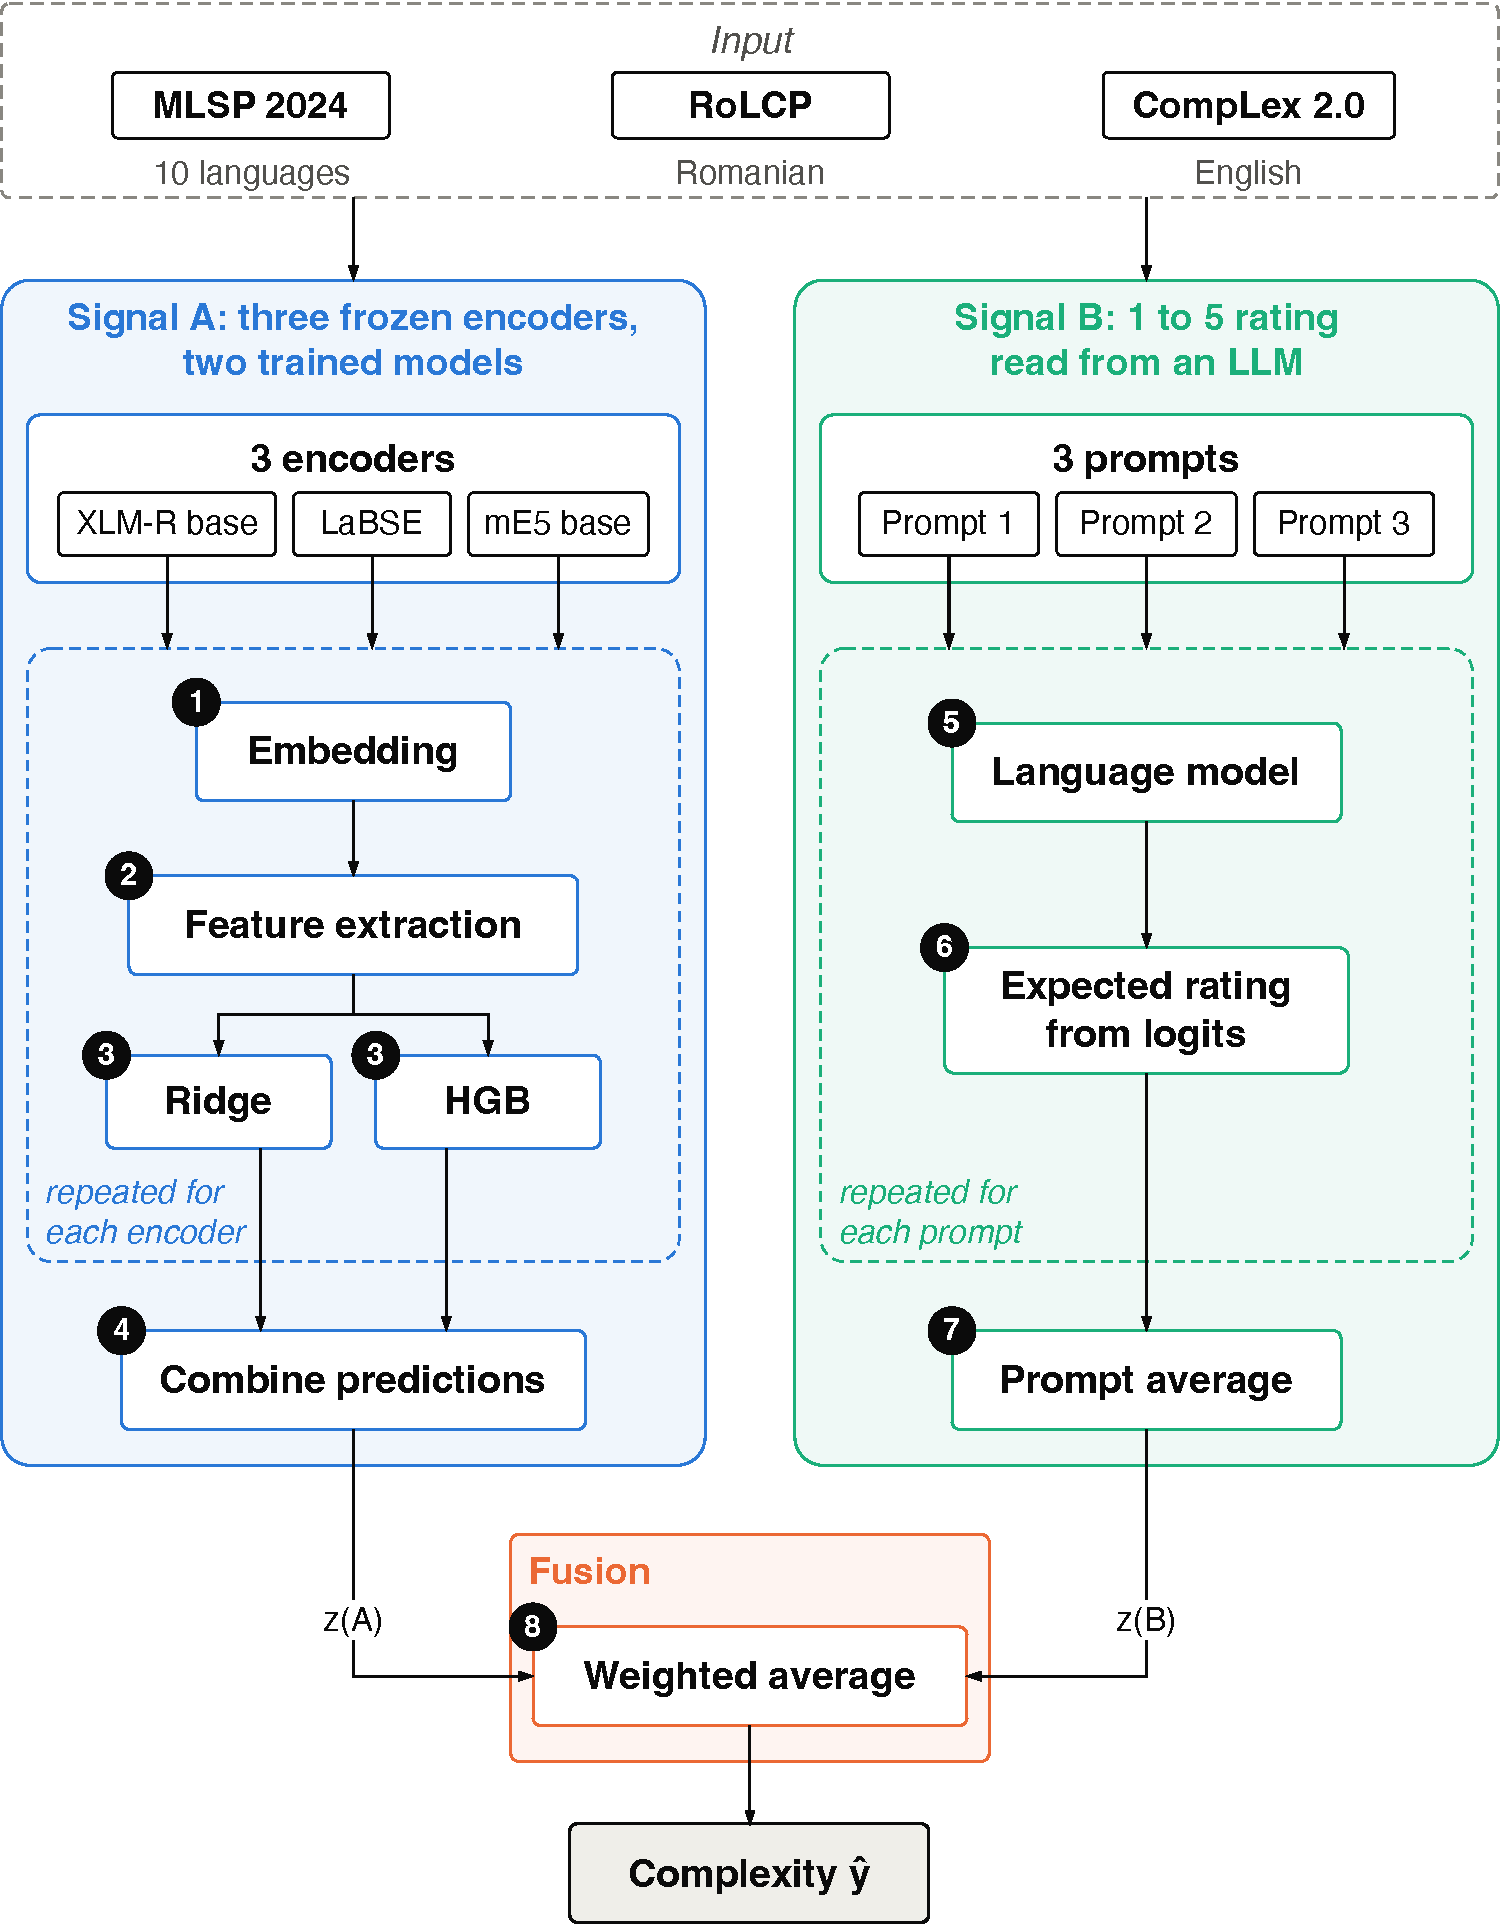
\includegraphics[width=0.77\textwidth]{fig_pipeline_doc_vertical.pdf}
\caption{The pipeline for one test language. The numbered circles are the steps described in
Sections~\ref{sec:signal-a} to~\ref{sec:fusion}.}
\label{fig:pipeline}
\end{figure*}

% Style follows RALS (Anghel et al., EMNLP 2025), revised after Alexandru's review of 10 Oct 2026.
We predict how complex a word is in its context without any labelled example from the word's
language. We evaluate with a leave-one-language-out (LOLO) protocol: we predict the scores of one % release/fuse.py:3-16
language, the test language, using only the labelled data of the other languages, and repeat this
for every language.

The prediction combines two signals (Figure~\ref{fig:pipeline}). Signal~A (steps 1 to 4) is a model
trained on top of three multilingual encoders. Signal~B (steps 5 to 7) comes from a large language
model that gives a rating from 1 to 5 to the target word. Then we fuse the results from both signals
in step 8. We do not update the weights of the encoders or of the language model with fine-tuning or % release/signal_a.py:48, 55 (eval, no_grad); signal_b.py:117-123 (forward pass only)
any similar technique: we use them as published. The only models we train are a ridge regression
and gradient-boosted trees, in step 3.

Five settings are chosen with the labelled data of the other languages: the weights $w_{\mathrm{src}}$ % release/fuse.py:3-16
and $w$ of steps 4 and 8, the temperature $T$ and the grouping of ratings of step 6, and the language
model of step 5. For each of them, we try several candidate values and keep the one that gives the
highest correlation on the other languages. All other settings, such as the number of trees in
step 3, have fixed values, the same for every language.

\subsection{Data}
\label{sec:data}

We use three datasets. All three are used to train signal~A, and the first two also for evaluation: % release/signal_a.py:143-151 (CompLex plus the other languages, Romanian included with --with-ro)
\begin{enumerate}
\item MLSP 2024 \citep{shardlow-etal-2024-bea} contains ten languages: Catalan, English, Filipino,
French, German, Italian, Japanese, Portuguese, Sinhala and Spanish. We use its test split, in the
cleaned release, with 5{,}624 instances. We do not use its trial split, which has 30 labelled % output/doc_counts.txt, "MLSP test rows: 5624"; release/data.py:49, HF MLSP2024/MLSP2024
instances per language. % release/data.py:81, only load_mlsp("test"); 30 rows per language in data/MLSP2024/*/multils_trial_*_lcp_labels.tsv
\item RoLCP \citep{anghel-etal-2025-rals} contains 1{,}587 Romanian instances. Together with MLSP % output/doc_counts.txt, row ro and "eval rows (11 langs): 7211"
2024, it gives 7{,}211 evaluation instances in eleven languages.
\item CompLex 2.0 \citep{shardlow-etal-2021-semeval} contains 8{,}423 English instances, from its % output/doc_counts.txt, "CompLex 2.0 rows: 8423"
single-word train, trial and test files. We use it only for training, not for evaluation. % release/data.py:33-34, COMPLEX_FILES
\end{enumerate}
Each instance consists of a context, a target word in it and a complexity score between 0 and 1. % output/doc_counts.txt, y_min and y_max
In all three datasets, annotators rated the target on a scale from 1 to 5, and the ratings were % Shardlow et al. 2024, Sec. 3 (1-5 scale); CompLex 2.0 uses the same 5-point scale
rescaled to $[0, 1]$ and averaged. Under LOLO, the MLSP 2024 and RoLCP instances of every language % RALS, Sec. 3.1 (rescaled to [0, 1] and averaged, following CompLex 2.0)
other than the test language are training data.

\subsection{Signal A}
\label{sec:signal-a}

Signal~A uses three multilingual encoders: XLM-R base \citep{conneau2020xlmr}, LaBSE % release/signal_a.py:29-32; fuse.py:211, default encoders
\citep{feng-etal-2022-language} and multilingual E5 base \citep{wang2024multilinguale5}. Steps 1 to
3 run separately for each encoder.

\paragraph{Step 1: Embedding.} Each encoder has its own tokeniser, which splits a text into tokens. % release/signal_a.py:46, 62
We give the tokeniser the whole context, cut to at most 500 characters on each side % release/data.py:35, 132-134
of the target. For every token, the tokeniser also returns the position of its characters in the % release/signal_a.py:62-65, return_offsets_mapping
text, so we can find the tokens that belong to the target word. A target can be one token or be
split into several. Each of the three encoders has 12 layers, and every layer computes an embedding % HF config.json of the three revisions: num_hidden_layers 12, hidden_size 768
of 768 numbers for every token. For each token of the target, we average its embeddings from the
last four layers. When the target has several tokens, its embedding is the average over these % release/signal_a.py:70, mean over layers (-4..-1), then over target tokens
tokens.

\paragraph{Step 2: Feature Extraction.} We centre the embeddings within each language. Centring
means shifting all the embeddings of a language by the same amount, so that their average becomes
zero. We compute the average embedding of all targets of the language and subtract it from the % release/signal_a.py:110-116, per_language
embedding of each target. We use only the instances of the language for this, not their labels.
CompLex is centred on its own average. Centring removes part of the information about which % release/signal_a.py:137-138
language an embedding comes from (Section~\ref{sec:tsne}).

We then add four word features, named as in the SHAP analysis of Section~\ref{sec:shap}: % release/signal_a.py:104-107, features; release/data.py:231-251, lexical
\begin{enumerate}
\item \emph{Subword count}, the number of tokens into which the XLM-R tokeniser splits the target, % release/data.py:254-258, fertility
a per-word version of the fertility of \citet{rust-etal-2021-good}. We use it to measure word
length. A character is a different unit in Japanese, Sinhala and Latin script, while the tokeniser
is the same for every language. The subword count is centred like the embeddings. % release/signal_a.py:104-107 (fert - language mean)
\item \emph{Word frequency}, the Zipf frequency from the wordfreq library \citep{speer-2022-wordfreq}, % release/data.py:213-219, zipf
which estimates how often a word is used from large collections of text in each language. The
scale is logarithmic: 3 means once per million words and 4 ten times per million. Many targets are % wordfreq README: Zipf = log10 of occurrences per billion words
inflected forms, such as plurals or conjugated verbs, which are rarer than their dictionary form,
the lemma. To avoid treating a rare form of a common word as a rare word, we look up both the word % release/data.py:238-244, lexical (max of form and lemma)
as written and its lemma and keep the higher frequency. The lemmas come from stanza
\citep{qi-etal-2020-stanza}, a library that analyses the grammar of a sentence, which we run on % release/data.py:138-195, lemmas (stanza on the full context)
the whole context. Stanza has no lemmatiser for Filipino, where we look up only the written form. % release/data.py:29, STANZA_LANGS
Words that wordfreq does not list get a frequency of 0. The library has no data for Sinhala, and all % release/data.py:200-219, freq_available and zipf
Sinhala targets have a frequency of 0. % output/doc_counts.txt, "frequency available": si False
\item \emph{Syllable count}, approximated by the number of groups of consecutive vowels. % release/data.py:222-228, n_syllables
\item \emph{Capitalised}, which is 1 when the word starts with a capital letter and 0 otherwise.
\end{enumerate}
Syllable count and capitalisation exist only for languages written in Latin script. Japanese and % release/data.py:26-27, 245-248, LATIN_SCRIPT
Sinhala have no capital letters, and their vowels are not separate letters that could be counted:
in Sinhala most vowels are signs attached to consonants, and Japanese kanji do not show how a word
is pronounced. For these two languages the two features are left empty. We also add two indicator % release/data.py:249-250
columns that mark the missing features: one is 1 for a language without word frequencies
(Sinhala), the other for a language not written in Latin script (Japanese and Sinhala). When such a % output/doc_counts.txt, frequency available
language is among the training languages, the indicators let the regressor tell its empty or zero
values apart from real ones.

\paragraph{Step 3: Ridge and HGB.} For each encoder, we train two models on the same data and % release/signal_a.py:91-101, blend_ridge_hgb
average their predictions. The first is a linear ridge regression with $\alpha = 300$, trained on
features standardised to mean 0 and standard deviation 1, with empty values replaced by the median. % release/signal_a.py:97-98
The second is histogram gradient-boosted trees (HGB), with 400 trees of depth 3, a learning rate of % release/signal_a.py:99-100
0.05 and an L2 penalty of 1.0. We call this average of the two models a regressor.

We train the regressor twice, on different data. The English regressor, $p_{\mathrm{en}}$, is
trained once on CompLex alone and predicts every language. The multilingual regressor, % release/signal_a.py:143
$p_{\mathrm{multi}}$, is trained on CompLex together with the labelled instances of the other
languages and is retrained for each test language. When English is the test language, we leave % release/signal_a.py:145-151
CompLex out of $p_{\mathrm{multi}}$ and replace $p_{\mathrm{en}}$ by $p_{\mathrm{multi}}$, so that % release/signal_a.py:147-148, 152
the regressors that predict English see no English label.

\paragraph{Step 4: Combine Predictions.} Each target now has six predictions: one from each of the
two regressors for each of the three encoders. Within each language, we standardise the predictions % release/fuse.py:42-68, load_a
of each regressor and encoder: we subtract their average and divide by their standard deviation.
This puts the three encoders on one scale and does not change the correlation with the ground-truth scores,
which is what we measure (Section~\ref{sec:protocol}). We then average the standardised predictions
over the three encoders, which gives one $p_{\mathrm{en}}$ and one $p_{\mathrm{multi}}$ for each
target. Signal~A is their weighted average:
\begin{equation}
A = w_{\mathrm{src}}\, z(p_{\mathrm{en}}) + (1 - w_{\mathrm{src}})\, z(p_{\mathrm{multi}}),
\label{eq:arms}
\end{equation}
where $z$ standardises within the language. The weight $w_{\mathrm{src}}$ says how much the % release/fuse.py:71-75, z_a
English regressor counts: with $w_{\mathrm{src}} = 1$, signal~A is the English regressor alone, with
$w_{\mathrm{src}} = 0$ the multilingual regressor alone, and with $w_{\mathrm{src}} = 0.75$ the
English regressor gets three quarters of the weight. The weight is not fixed: we try nine values,
$0, 0.125, 0.25, \dots, 1$, and keep the one that works best on the other languages, together with % release/fuse.py:38, SRC_GRID
the weight of step 8 (Section~\ref{sec:fusion}).

\subsection{Signal B}
\label{sec:signal-b}

\paragraph{Step 5: Language Model.} We give the large language model the context and the target and % release/signal_b.py:60-70, PROMPTS
ask it for a single digit, from 1 (very familiar) to 5 (very difficult). We do this with three
prompts. All three are written in English, name the language of the context and contain no example % release/signal_b.py:60-70, PROMPTS
with a known score. They differ in wording: the first asks the model to answer as an expert in the
language's linguistics, the second is a short instruction, and the third marks the target inside % release/signal_b.py:138-147, render
the context with \guillemotleft\,\guillemotright. We use three prompts because the rating of a
single prompt depends on its wording, and prompts with different wording make partly different
errors, which their average reduces. The model writes no text: we run it once per prompt and read % release/signal_b.py:117-135, logits, digit_probs
the probabilities it gives to the first token of its answer.

\paragraph{Step 6: Expected Rating from Logits.} A language model writes its answer one token at a
time. Before writing a token, it gives a score, called a logit, to every token in its vocabulary,
and these scores are turned into probabilities that sum to one. We read the probabilities of the
first token of the answer and keep only those of the five tokens \texttt{1} to \texttt{5}. The model % release/signal_b.py:125-135, digit_probs
also gives some probability to other tokens, so we divide the five by their sum to make them sum to
one. The result says how likely the model finds each rating. Instead of keeping only the most likely
rating, we take the expected rating, the average of the five ratings weighted by their
probabilities. Unlike the most likely rating, it also reflects how unsure the model is between
consecutive ratings.

Before taking the expected rating, we change the probabilities in two ways. First, a temperature
$T$ controls how spread out they are: each probability is raised to the power $1/T$, and the five % release/fuse.py:79-83, temper
are again divided by their sum. With $T > 1$ the distribution becomes more random, closer to five
equally likely ratings, and with $T < 1$ it becomes more deterministic, closer to the single most
likely rating. Second, we merge consecutive ratings into groups. A group counts as a single % release/fuse.py:33-35, PARTITIONS; 86-88, b_of
rating: its value is the mean of its ratings, and its probability is the sum of their
probabilities. We use the grouping $\{1\}, \{2, 3\}, \{4, 5\}$, with values 1, 2.5 and 4.5. We % doc_fuse_ro11.txt, partition 1|23|45 for all 11 languages
tested all 15 possible groupings, and for every test language this one had the highest score on % release/fuse.py:34-35, 104-108: 15 partitions, chosen by mean r over the other languages
the other languages. The rating for prompt $k$ is the expected rating, rescaled from the
range 1 to 5 to the range 0 to 1 of the ground-truth scores:
\begin{equation}
B_k = \frac{1}{4}\Big(\sum_{g} P_g\, v_g - 1\Big),
\label{eq:rating}
\end{equation}
where $g$ runs over the groups and $P_g$ and $v_g$ are the probability and the value of group $g$. % release/fuse.py:89

\paragraph{Step 7: Prompt Average.} Steps 5 and 6 give one rating $B_k$ for each of the three % release/fuse.py:88-89, b_of (np.mean over prompts)
prompts. The score of signal~B is their arithmetic mean, $B = (B_1 + B_2 + B_3)/3$.

\paragraph{Choosing the Settings of Signal B.} The language model never sees a label. We use the % release/fuse.py:92-110, build_b
labels of the other languages only to choose three settings, one after the other. For each
candidate, we compute signal~B on every other language, measure its correlation with the
ground-truth scores there and average these correlations; the candidate with the highest average is kept. We
choose: (1) the temperature $T$, among 16 values from 0.5 to 64, with no grouping applied; (2) the grouping, % release/fuse.py:32, T_GRID; 98-100, pick_t on the neutral partition
among the 15 groupings of step 6; and (3) % release/fuse.py:34-35, 104-108
 the language model, among three models with openly published % release/fuse.py:165-171, pick_model
weights: Gemma~4 12B \citep{gemmateam-2026-gemma4}, Qwen3 8B \citep{yang-etal-2025-qwen3} and % release/signal_b.py:38-49, MODELS
Qwen3.5 9B. Gemma~4 and Qwen3 are quantised to 4 bits, and Qwen3.5 to 8 bits. % release/signal_b.py:30-49, MODELS; Qwen limits (no T, grouping, third prompt: fuse.py:142-145) are stated in Results; Qwen on Romanian: output/doc_ablations_qwen_ro.txt (not in release/predictions)

\subsection{Fusion}
\label{sec:fusion}

\paragraph{Step 8: Weighted Average.} We standardise $A$ and $B$ within the language and fuse them
with a weighted average:
\begin{equation}
\hat{y} = w\, z(A) + (1 - w)\, z(B),
\label{eq:fusion}
\end{equation}
where $w$ is the weight of signal~A and $1 - w$ the weight of signal~B. The result, $\hat{y}$, is the predicted % release/fuse.py:37, W_GRID (0, 0.05, ..., 1); 238-239
complexity score.

We choose $w_{\mathrm{src}}$ and $w$ on the other languages by repeating the LOLO protocol among % release/fuse.py:191-205, fit
them. For each candidate $w_{\mathrm{src}}$, we set aside each other language once, choose $w$ on
the remaining ones and record the correlation on the language set aside. We keep the
$w_{\mathrm{src}}$ with the highest average correlation, and then choose $w$ on all the other
languages. For these choices, the signals of each other language are its own LOLO predictions. % release/fuse.py:174-188, signals; 233

\subsection{Evaluation Protocol}
\label{sec:protocol}

For each test language, the multilingual regressor, $w_{\mathrm{src}}$, $T$, the grouping, the
language model and $w$ are trained or chosen on the other languages only. The test language
contributes its instances without labels, to centre its embeddings and subword counts in step~2 and % release/signal_a.py:110-116
to standardise its predictions. % release/fuse.py:65, 75, 185

The labels of the test language are never used to make its own predictions. They have one indirect
effect. $w_{\mathrm{src}}$, $w$ and the language model are chosen from the predictions on the other % release/fuse.py:14-16
languages, and those predictions were made with the test language in the training data, for
signal~A and for the choice of $T$ and of the grouping. The labels of CompLex have the same indirect
effect on English.

We measure the Pearson correlation between the predicted and the ground-truth complexity scores on each % release/data.py:262-268, pearson
language, and report the average of these correlations over the languages. To show how much a % release/fuse.py:259-260
correlation depends on the particular contexts in the test data, we report a 95\% confidence
interval computed with a bootstrap. Several targets often share a context, so we resample whole % release/data.py:281-294, boot_r
contexts, each with all its targets, rather than single targets. For each language, we draw 2{,}000 % release/fuse.py:214, --boot 2000
bootstrap samples, each made of as many contexts as the language has, drawn at random with
replacement, and compute the correlation on each sample. The interval goes from the 2.5th to the
97.5th percentile of these 2{,}000 correlations. For the average over languages, we average the % release/fuse.py:241-256
correlations of the first sample of every language, then those of the second sample, and so on, and
take the same percentiles of these 2{,}000 averages.

% =====================================================================
\section{Experimental Results}
\label{sec:results}
% Sources: output/doc_fuse_ro11.txt (fuse.py --with-ro), output/doc_fuse_mlsp10.txt (fuse.py),
% output/doc_ablations.txt (every fuse.py ablation), output/doc_ablations_extra.txt
% (analysis_doc_ablations_extra.py: the ablations fuse.py has no flag for, the Qwen rows on 11
% languages, and paired bootstrap intervals), output/doc_correlations.txt
% (analysis_doc_correlations.py). Development runs: output/e_extractie.md (layers) and
% output/e_bakeoff.md (language models on the trial split). Three-decimal values were rounded from a
% full-precision rerun of the same command; they match the four-decimal files.
% Order since 11 Oct 2026, asked by Alexandru: signal A, signal B, fusion, published results.

All results follow the LOLO protocol of Section~\ref{sec:protocol}. It applies to both signals. % release/fuse.py:3-16, 226-237
The ridge regression and HGB of signal~A are trained on the labelled instances of the other % release/signal_a.py:143-151
languages in the dataset, never on those of the test language. Signal~B does not fine-tune the
language model or use any similar technique. Its temperature, grouping and language model are % release/fuse.py:92-110, 165-171
chosen on the other languages, and so is the weight $w$ of the fusion. The % release/fuse.py:191-205
labels of the test language are used only to compute the correlations that we report. Three
comparisons come from runs made before the final experiments: the encoder layers and TabFM in
Section~\ref{sec:results-a}, and the first comparison of language models in
Section~\ref{sec:results-b}.

To see whether a difference from the full method is larger than chance, we compute it on each of % analysis_doc_ablations_extra.py, paired: data.boot_r has a fixed seed, so resample k is the same contexts in every run (0 degenerate resamples; reproduced on 10 Oct 2026 with fuse.py copies edited in the file and an own bootstrap)
the 2{,}000 bootstrap samples of Section~\ref{sec:protocol} and report the 95\% interval of these
differences. When the interval excludes zero, the difference is unlikely to come from the particular
test contexts. Mean is the average over the eleven languages.

\subsection{Signal A}
\label{sec:results-a}

\begin{table}[t]
\centering
\small
\setlength{\tabcolsep}{2.5pt}
% doc_ablations.txt (encoders, fuse.py --with-ro --encoders ...) and doc_ablations_extra.txt (w_src
% fixed, from the stored predictions with the rest of fuse.py unchanged); A and fused, 11 languages.
% The correlations between the single encoders (doc_correlations.txt, part 5) are given in the text;
% until 11 Oct 2026 they were columns (1), (2) of this table.
\begin{tabular}{lcc}
\toprule
 & Signal A & Fused \\
\midrule
\textbf{Full method}              & \textbf{.610} & \textbf{.693} \\ % 0.609568 / 0.692521
\midrule
XLM-R base only                   & .590 & .688 \\ % 0.590287 / 0.687851
LaBSE only                        & .587 & .690 \\ % 0.586871 / 0.689799
Multilingual E5 base only         & .591 & .689 \\ % 0.591327 / 0.689233
Plus XLM-R large                  & .619 & .694 \\ % 0.618583 / 0.694246
\midrule
English regressor only            & .605 & .693 \\ % w_src = 1: 0.605280 / 0.692576
Multilingual regressor only       & .606 & .689 \\ % w_src = 0: 0.606162 / 0.689273
\bottomrule
\end{tabular}
\caption{Signal~A and the fusion when one part of signal~A is changed. Mean Pearson correlation
over the eleven languages.}
\label{tab:signal-a}
\end{table}

\paragraph{Encoders.} Signal~A uses three encoders. We first ran signal~A with each encoder alone % release/fuse.py --encoders
(Table~\ref{tab:signal-a}). With a single encoder, signal~A reaches 0.587 to 0.591 and the fusion % 0.586871 / 0.590287 / 0.591327; fused 0.687851 / 0.689799 / 0.689233
0.688 to 0.690. We then computed the Pearson correlation between the signal~A of each pair of
encoders, within each language. XLM-R base and LaBSE correlate at 0.870, and multilingual E5 correlates % doc_correlations.txt, part 5: XLM-R--LaBSE 0.870, XLM-R--mE5 0.890, LaBSE--mE5 0.890
at 0.890 with each of the other two. Each encoder therefore makes partly different errors. We
average the three (step~4 in Figure~\ref{fig:pipeline}). The average gives a better result than any % release/fuse.py:42-68, load_a
single encoder: signal~A rises by 0.018 to 0.023 and the fusion by 0.003 to 0.005, and each % A: 0.609568 - 0.590287 / 0.586871 / 0.591327 = 0.0193 / 0.0227 / 0.0182; fused: +0.0047, +0.0027, +0.0033
interval of the gain in the fusion excludes zero. A fourth encoder, XLM-R large % doc_ablations_extra.txt, 11 languages: the three single-encoder intervals exclude zero
\citep{conneau2020xlmr}, raises signal~A by 0.009 and the fusion by 0.002. On the ten MLSP % A +0.0090; fused +0.0017 [+0.0005, +0.0030]
languages, in the run without Romanian of Section~\ref{sec:published}, this gain in the fusion % 10 languages: +0.0001 [-0.0010, +0.0012]
disappears and its interval includes zero.

\paragraph{Encoder Layers.} Each encoder has 12 layers, and we average the embeddings of the last % release/signal_a.py:70, layers -4..-1
four (step~1 in Figure~\ref{fig:pipeline}). We chose the layers in development, with an earlier version of the method: XLM-R base % output/e_extractie.md (analysis_extractie.py): XLM-R base only, multilingual regressor (p_multi), 10 MLSP languages, fusion of that time (0.680 with the last four layers)
alone, the multilingual regressor and the ten MLSP languages. We compared four options: the last % solution_bert.py:75-92, EMB_CONFIGS: last4 (-4..-1, mean), mid (6..9, mean), concat4 (-4..-1, concatenated), last1 (-1)
four layers averaged, layers 6 to 9 averaged, the last four layers joined into one vector of
3{,}072 numbers, and the last layer alone. The last four layers averaged gave the highest % e_extractie.md, mean pooling: last4 0.5778, mid 0.5720, concat4 0.5708, last1 0.5691
signal~A, 0.578 against 0.569 to 0.572. With the other options the fusion was lower by less than % fused vs last4: mid -0.0017 [-0.0039, +0.0005], concat4 -0.0006 [-0.0026, +0.0014], last1 -0.0010 [-0.0032, +0.0013]
0.002, and every interval of this difference included zero.

\paragraph{Embedding Centring.} In step~2 we centre the embeddings within each language. For a % release/signal_a.py:110-116, per_language: E[m] - E[m].mean(0)
target $i$ of language $L$ with embedding $e_i$, the centred embedding is
\begin{equation}
\tilde{e}_i = e_i - \frac{1}{n_L} \sum_{j \in L} e_j,
\label{eq:centring}
\end{equation}
where the sum runs over the $n_L$ targets of $L$. Centring is a simple form of domain adaptation
without labels: each language is a domain, and centring gives all domains the same average
embedding, as in \citet{libovicky-etal-2020-language}.
\label{sec:tsne}

% Neighbour shares recomputed on 9 Oct 2026, and again on 10 Oct, from
% data/emb_mlsp10_{xlmr,labse,e5}_last4_7211.npy with the procedure of output/umap_concat3.py
% (cosine distance, same-sentence targets left out): 0.5668 before, 0.3298 after, chance (sum of
% squared language shares) 0.1096. Before centring: fil 0.83, ja 0.84, si 0.94.
% Figure: output/tsne_centrare_3encodere_concat_fara_knn.png (output/tsne_concat_fara_knn.py: same
% projection as output/tsne_3encodere.py, without the neighbour-share line and, since 10 Oct, without
% the figure title; fonts doubled and legend on two rows, same projection).
\begin{figure*}[t]
\centering
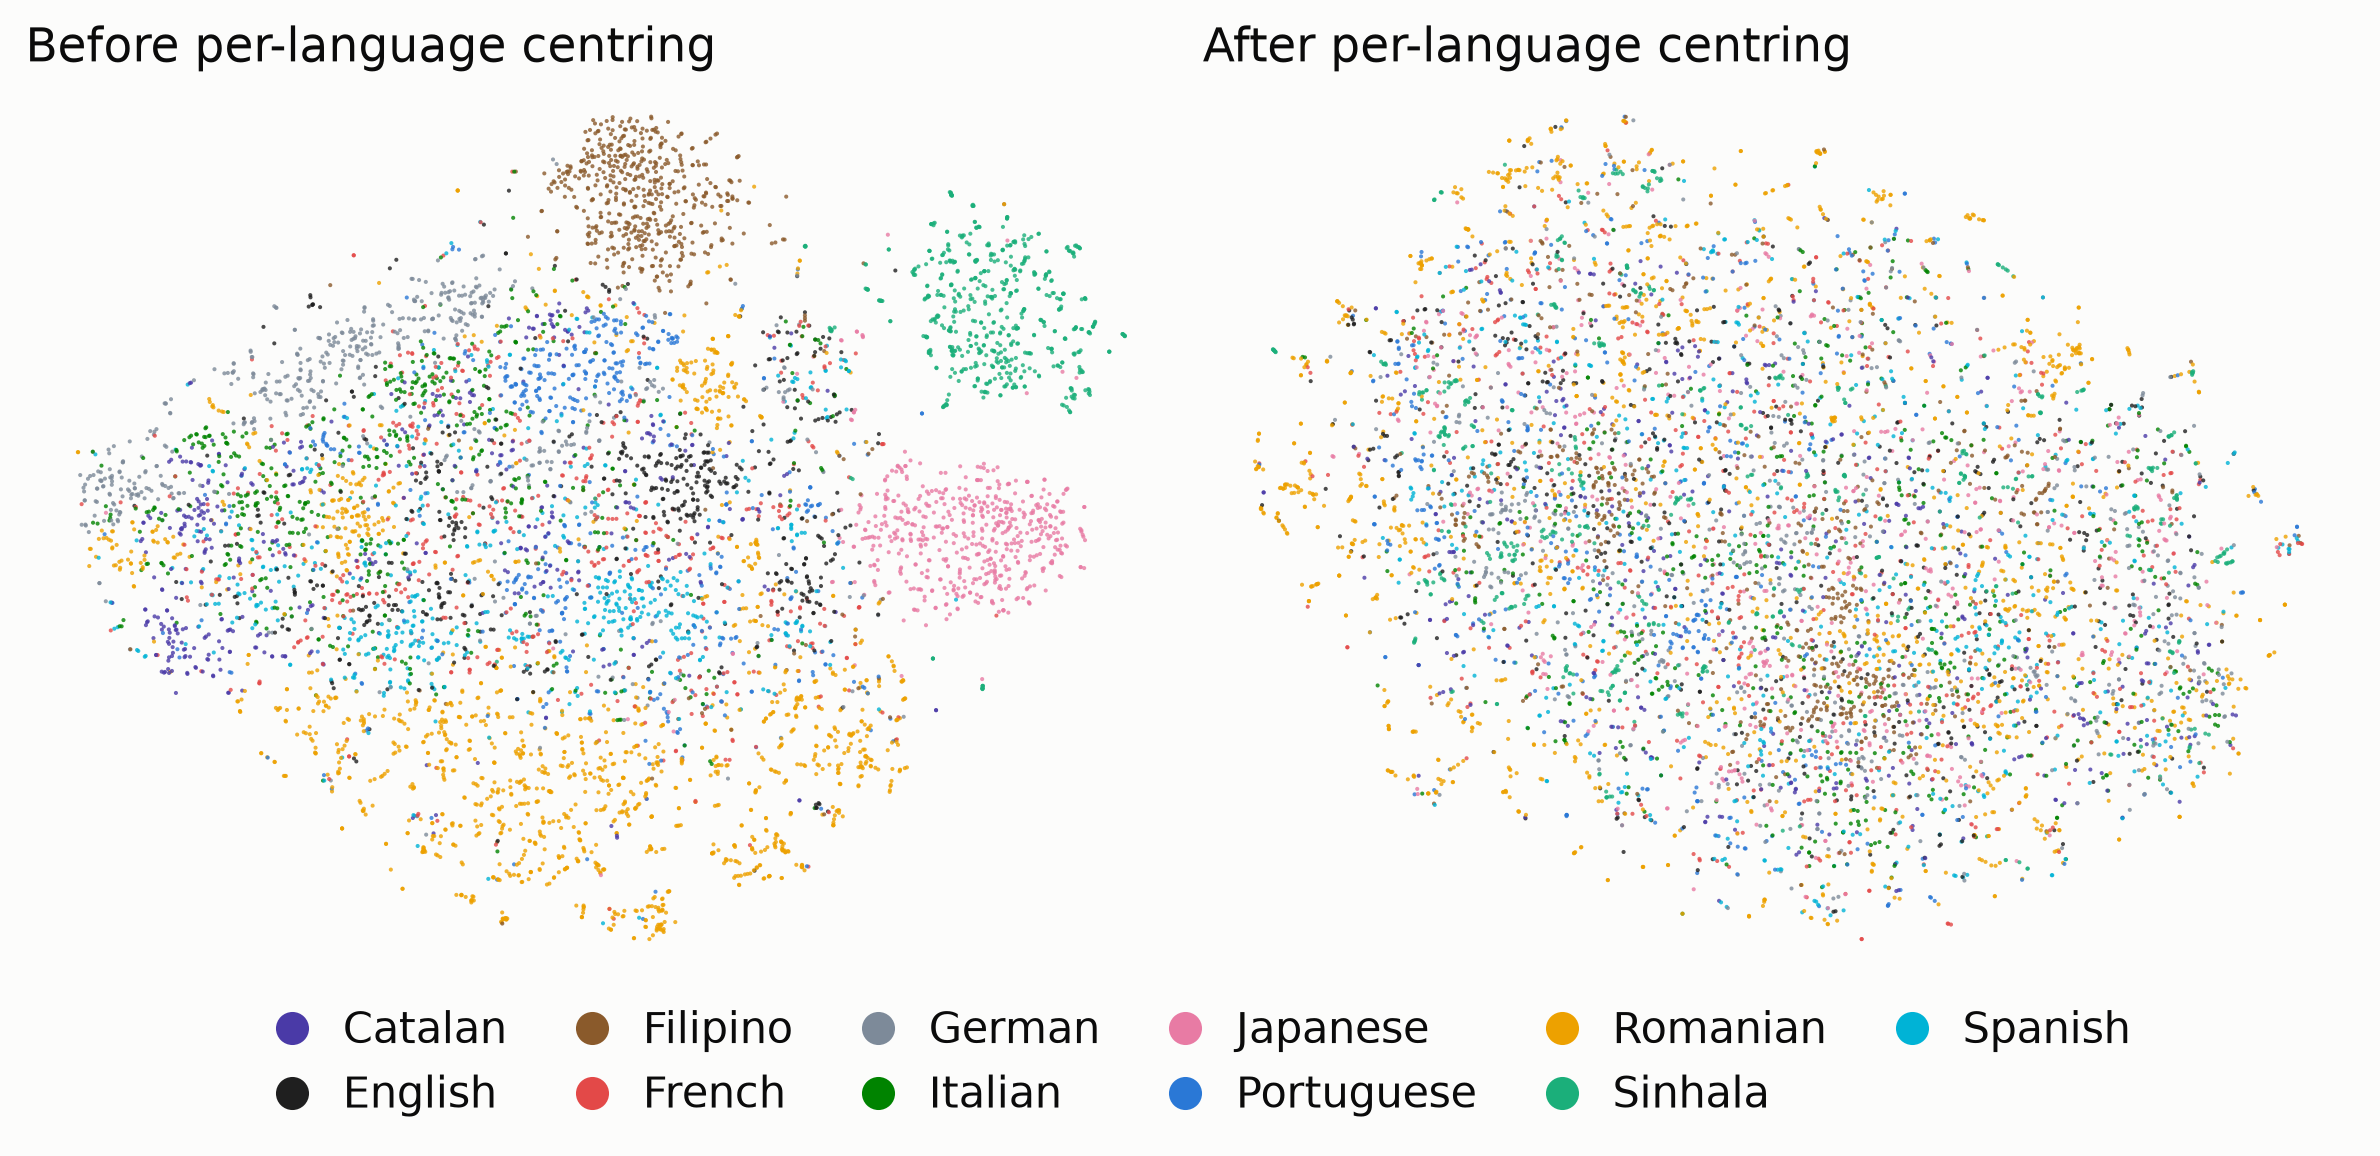
\includegraphics[width=\textwidth]{fig_tsne_encoders.png}
\caption{t-SNE of the target embeddings of the 7{,}211 instances, before and after per-language
centring. The embeddings of XLM-R base, LaBSE and multilingual E5 base are joined into one vector, % output/tsne_concat_fara_knn.py, bloc: each block divided by its root mean squared norm
each scaled to the same total variance (PCA to 50 dimensions, perplexity 30, seed 0).}
\label{fig:tsne}
\end{figure*}

Figure~\ref{fig:tsne} shows what the centring of step~2 removes. It uses t-SNE
\citep{vandermaaten-hinton-2008-tsne}, which draws high-dimensional vectors as points in a plane
and keeps vectors that are close in the original space close in the plane. The coordinates of the
three encoders mean different things and cannot be averaged. We join the three embeddings of a
target into one vector instead, and project these vectors before and after centring. Before
centring, Filipino, Japanese and Sinhala form clusters of their own. After centring, these clusters
disappear and the languages mix. A regressor trained on the other languages could therefore find it
easier to predict the test language, but we did not measure this.
% The share of the 15 nearest neighbours from the same language (0.57 before, 0.33 after, 0.11 at
% random; output/umap_concat3.py) was in the text until 11 Oct 2026, removed at Alexandru's request.
% Signal A without centring was never run.

\paragraph{Regression models.} In step~3, we train two models on the features of each encoder, a
ridge regression and HGB, and average their predictions with equal weights. % release/signal_a.py:101, np.mean over (ridge, hgb)

\begin{table}[t]
\centering
\small
\setlength{\tabcolsep}{4pt}
% output/doc_signal_a_models.txt (analysis_doc_signal_a_models.py): each model replaces the average of
% ridge and HGB in step 3, with the hyperparameters of the development runs (solution_bert.py), the
% rest of the method unchanged, 11 languages. Ridge + HGB reproduces release/predictions/signal_a.csv
% exactly (max |diff| 0.00e+00) and gives 0.692521 again. The correlation matrix between the models
% is in the same file; the table showed it until 11 Oct 2026.
\begin{tabular}{lcc}
\toprule
Model & Signal A & Fused \\
\midrule
\textbf{Ridge + HGB (ours)} & \textbf{.610} & \textbf{.693} \\ % r_A 0.609568, fused 0.692521
\midrule
Ridge                & .603 & .690 \\ % r_A 0.603368, fused 0.689860, vs ours -0.0027 [-0.0048, -0.0005]
HGB                  & .588 & .690 \\ % r_A 0.588084, fused 0.690434, vs ours -0.0021 [-0.0043, +0.0003]
LightGBM             & .587 & .690 \\ % r_A 0.586553, fused 0.690137, vs ours -0.0024 [-0.0047, +0.0002]
XGBoost              & .587 & .690 \\ % r_A 0.586687, fused 0.689753, vs ours -0.0028 [-0.0050, -0.0004]
CatBoost             & .588 & .690 \\ % r_A 0.588477, fused 0.690222, vs ours -0.0023 [-0.0049, +0.0004]
ExtraTrees           & .588 & .687 \\ % r_A 0.588000, fused 0.686729, vs ours -0.0058 [-0.0085, -0.0032]
RandomForest         & .576 & .685 \\ % r_A 0.575584, fused 0.685342, vs ours -0.0072 [-0.0102, -0.0043]
MLP                  & .570 & .686 \\ % r_A 0.569643, fused 0.685914, vs ours -0.0066 [-0.0101, -0.0028]
% kNN (k = 50) was also run: r_A 0.445483, fused 0.671035, vs ours -0.0215 [-0.0269, -0.0163]; replaced
% by TabFM on 11 Oct 2026, asked by Alexandru.
\midrule
% Development run, TabFM on a T4 GPU (n_estimators 8, max_num_features 256), XLM-R base only, embedding
% projected on its first 394 principal components (finetune_xlmr.py:300-306, emb_transform proj-N), ten
% MLSP languages, fuse_ab.py --arm lolo --fit test --pick-split test --b-dir output/bakeoff_test_M3K.
% Signal A here is the multilingual regressor alone; values compare only within these three rows.
Ridge + HGB         & .575 & .680 \\ % output/e_fusion_lolo_ctrl_proj394.md: A 0.5749, fused 0.6803
TabFM                & .567 & .678 \\ % output/e_fusion_lolo_doc_tabfm_alone_mf256.md (11 Oct 2026): A 0.5673, fused 0.6783, vs ridge + HGB -0.0019 [-0.0042, +0.0003]
Ridge + TabFM        & .579 & .681 \\ % output/e_fusion_lolo_rt_mf256_vsctrl.md: A 0.5790, fused 0.6806, vs ridge + HGB +0.0003 [-0.0012, +0.0018]
\bottomrule
\end{tabular}
\caption{Signal~A and the fusion with each model of step~3. Mean Pearson correlation over the
languages. The last three rows come from a smaller run and compare only with each other.}
\label{tab:signal-a-models}
\end{table}

In step~3 we also replaced the average of the ridge regression and HGB by a single other model, % analysis_doc_signal_a_models.py, predict()
with the same features and the rest of the method unchanged. We tried ridge and HGB alone, two
other libraries of gradient-boosted trees, LightGBM and XGBoost, and CatBoost, whose trees use the
same split for all nodes of a level. The boosted trees have the same size as HGB: 400 trees of % LightGBM num_leaves 8, max_depth 3; CatBoost depth 3; XGBoost max_depth 3; all learning rate 0.05, 400 trees, L2 1.0
depth 3 and a learning rate of 0.05. We also tried ExtraTrees and RandomForest, which average many % ExtraTrees 500 trees, RandomForest 300 trees, max_features 0.3
deep trees, and a neural network with one hidden layer of 128 units (MLP). % MLP alpha 1e-3, early stopping
Results are in Table~\ref{tab:signal-a-models}.

The average of ridge and HGB gives the best signal~A and the best fusion. Every single model loses % doc_signal_a_models.txt, "fused vs ours"
in the fusion: 0.002 to 0.003 for ridge and the boosted trees, and 0.006 to 0.007 for ExtraTrees, % -0.0027, -0.0021, -0.0024, -0.0023, -0.0028; -0.0058, -0.0072, -0.0066
RandomForest and the MLP. For HGB, LightGBM and CatBoost the interval of this % intervals including zero: HGB [-0.0043, +0.0003], LightGBM [-0.0047, +0.0002], CatBoost [-0.0049, +0.0004]
loss includes zero. The boosted trees make almost the same predictions: their signal~A correlates % doc_signal_a_models.txt, correlation matrix: boosted trees 0.974-0.995
at 0.974 to 0.995. Ridge correlates with them at only 0.88. Between ridge and HGB, the % ridge with HGB 0.883, LightGBM 0.881, XGBoost 0.884, CatBoost 0.884
correlation is lowest on Sinhala, 0.571, and between 0.831 and 0.957 on the other languages % doc_correlations.txt, part 4: si 0.5708, ca 0.8311, fil 0.9573
(Table~\ref{tab:corr-ab}). The average of ridge and HGB is better
than either of them: it combines two models that make partly different errors.

We also tried TabFM, a tabular foundation model from Google Research. TabFM fits no parameters: it % TabFM, google-research/tabfm (July 2026); bib entry still needed
reads the training rows as context and predicts each new row from them, and it averages 8 such % n_estimators 8 (tabfm_colab.ipynb, setari.json)
predictions. We ran TabFM on fewer dimensions. Before step~3, we reduced the embedding from 768 to % TabFM on a T4 GPU: the full 768-dimensional embedding did not fit in its 16 GB
394 dimensions with principal component analysis (PCA), which keeps the directions along which the % finetune_xlmr.py:300-306, proj-394: PCA on all embeddings, no label
embeddings vary most. This run was made before the final experiments, with XLM-R base alone, the
multilingual regressor alone and the ten MLSP languages. The last three rows of
Table~\ref{tab:signal-a-models} compare TabFM with ridge and HGB in this run. TabFM alone lowers the % e_fusion_lolo_doc_tabfm_alone_mf256.md: -0.0019 [-0.0042, +0.0003]
fusion by 0.002, and ridge with TabFM raises it by less than 0.001. Both intervals include zero. % e_fusion_lolo_rt_mf256_vsctrl.md: +0.0003 [-0.0012, +0.0018]

% Defined here so that the figure lands on the page of the SHAP text below.
% Values: output/shap_signal_a_per_encoder_importance.csv and _correlations.csv
% (analysis_shap_signal_a_per_encoder.py, the computation of analysis_shap_signal_a.py with the
% embedding split by encoder). Signal A in output/shap_signal_a_per_encoder_raw.npz equals column A
% of output/doc_fuse_ro11.csv to 1.3e-15.
\begin{figure*}[t]
\centering
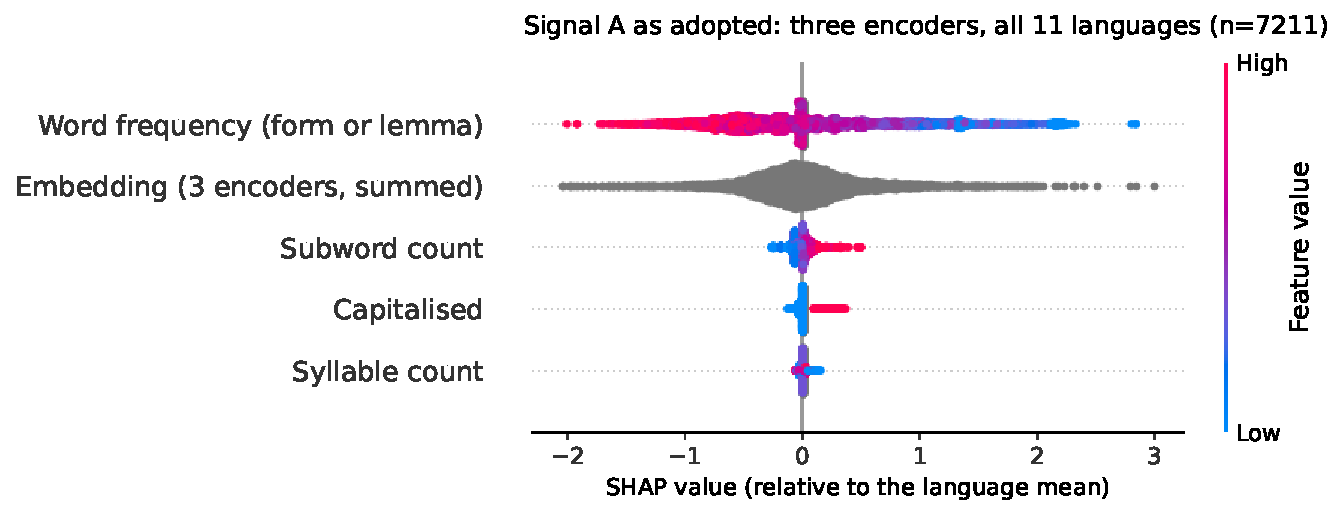
\includegraphics[width=0.7\textwidth]{fig_shap_signal_a.pdf}
\caption{SHAP values of the four word features of signal~A for the 7{,}211 instances, in standard
deviations of signal~A within the instance's language. Colour is the feature value. The embeddings
are shown in Figure~\ref{fig:shap-all} (Appendix~\ref{sec:appendix-shap}).}
\label{fig:shap}
\end{figure*}

\paragraph{English and multilingual regressors.} Signal~A mixes two regressors, trained on different % release/signal_a.py:143-151
data (step~4). The English regressor is trained only on CompLex, the largest dataset, with 8{,}423 % output/doc_counts.txt, "CompLex 2.0 rows: 8423"
English instances. It sees no other language, and the same model predicts every test language. The % release/signal_a.py:143, p_en_all = blend_ridge_hgb(Xen, yen, X)
multilingual regressor is trained on CompLex together with the labelled MLSP 2024 and RoLCP
instances of the ten languages other than the test language. It sees words from many languages, % release/signal_a.py:145-151, retrained for each L
but it has to be trained again for each test language. We use both because they learn from
different data and make partly different errors. The last two rows of Table~\ref{tab:signal-a} use
each regressor alone. With the
English regressor alone, signal~A falls by 0.004, and the fusion changes by less than 0.001, with % A -0.0043; fused +0.0001 [-0.0009, +0.0010]
an interval that includes zero. The full method already gives the English regressor most of the
weight: $w_{\mathrm{src}}$, chosen on the other languages, is between 0.625 and 1. With the % doc_fuse_ro11.txt, column w_src
multilingual regressor alone, signal~A and the fusion both fall by 0.003, and the interval of the % A -0.0034; fused -0.0032 [-0.0057, -0.0008]
difference in the fusion excludes zero.

\paragraph{Word features.} Besides the embeddings, signal~A has four word features (step~2): % release/data.py:231-258
\emph{Word frequency}, \emph{Subword count}, \emph{Syllable count} and \emph{Capitalised}. We chose
features that need no label. The ridge regression baseline of RALS for RoLCP uses the same kinds of % RALS, Results, "Lexical Complexity Prediction": zipf_frequency, character length, vowels, syllables (pyphen), is title, ...
features: Zipf frequency, word length, syllable count and whether the word is capitalised
\citep{anghel-etal-2025-rals}. We count length in subwords instead of characters, because a
character is a different unit in Japanese, Sinhala and Latin script.
\label{sec:shap}

Figure~\ref{fig:shap} shows which inputs signal~A relies on, measured with SHAP values
\citep{lundberg-lee-2017-unified}. The reference is the average of signal~A over the instance's % analysis_shap_signal_a.py:120-121, background = all rows of the explained language
language.
% Exact SHAP: A is affine in the six regressor predictions within a language
% (analysis_shap_signal_a.py:165-188); ridge in closed form, HGB with interventional TreeSHAP
% (lines 107-124). The two indicator columns are constant within a language and get 0 (importance.csv).

\emph{Word frequency} is the strongest input. On average it moves signal~A by 0.56 of its standard % importance.csv, all: frequency 0.5566
deviation within the language. Frequent words are pushed towards simple, rare words towards
complex. The embedding of each encoder moves signal~A by 0.12 to 0.13, and the three embeddings % importance.csv, all: mE5 0.1303, XLM-R 0.1258, LaBSE 0.1194; three embeddings together 0.3144
together by 0.31. The total is less than the sum of the three, because for many instances one % "together" = mean |sum of the three|, analysis_shap_signal_a_per_encoder.py:103-105 (emb_all); sum of the three 0.3755
encoder pushes signal~A up while another pushes it down. \emph{Subword count}, \emph{Capitalised} % shap_signal_a_per_encoder_raw.npz: the three encoder contributions differ in sign for 48% of instances (10 Oct 2026)
and \emph{Syllable count} each stay below 0.06. \emph{Capitalised} matters mainly in German % importance.csv: subword 0.0566, capitalised 0.0213, syllables 0.0158
(0.097). On Sinhala, the three embeddings together move signal~A by 0.81 and \emph{Subword count} % importance.csv: capitalised de 0.0970
by 0.15. The Spearman correlation between the SHAP contribution of an input and ground-truth % importance.csv, si: embeddings together 0.8052, subword 0.1494
complexity, computed within each language, gives the same order: 0.57 for \emph{Word frequency}, % correlations.csv, rho_contribution: frequency 0.5748 (10 languages), XLM-R 0.3780, mE5 0.3633, LaBSE 0.3476, syllables 0.0621 (9 languages)
0.35 to 0.38 for the embeddings and 0.06 for \emph{Syllable count}.

\subsection{Signal B}
\label{sec:results-b}

\paragraph{Baseline.} We also built a baseline with current foundation models. We first tested Claude Sonnet 5.5 and % output/doc_claude_baseline.txt
Claude Opus 5.5 as standalone models: each model rated the complexity of every test instance,
zero-shot and with the same prompt. Sonnet reached 0.685 on eleven languages and 0.675 on ten, below
our method by 0.008 and 0.015, and close to signal~B alone (0.663 and 0.665). Opus reached 0.721 % .693 - .685, 0.689745 - 0.6747
and 0.711, above our method by 0.028 and 0.021. We then fused each Claude model with our already % .721 - .693, 0.7111 - 0.689745
trained method, with a weighted average as in step~8. With Sonnet, the fusion reached 0.706 on the % doc_claude.txt (11 Oct, recomputed on release/ predictions), 10 languages: method + sonnet 0.706484, method + opus 0.724129
ten MLSP languages. With Opus, it reached 0.724, 0.013 more than Opus alone. Fusing Sonnet with % doc_claude.txt, 10 languages: method + opus - opus +0.0130 [+0.0094, +0.0170]
Opus gave almost no gain, 0.001. % doc_claude_baseline.txt: Opus + Sonnet 0.7117 - 0.7111 = 0.0006 (not recomputed)
Table~\ref{tab:ablations} gives the results on eleven languages next to our two signals and the
full method. In its last two rows, the rating of the Claude model replaces signal~B in the fusion.
With signal~A, Opus reaches 0.725 and Sonnet 0.695 on eleven languages. This is 0.004 above Opus % doc_claude.txt, 11 languages: A + opus 0.724900, A + sonnet 0.694997
alone and 0.010 above Sonnet alone, and both intervals exclude zero. With Gemma~4, the same % A + opus - opus +0.0037 [+0.0018, +0.0056]; A + sonnet - sonnet +0.0101 [+0.0064, +0.0137]
fusion adds 0.029 to signal~B (Section~\ref{sec:results-fusion}). The ratings of Opus and of % doc_ablations_extra.txt, signal B only vs full: -0.0290
Sonnet both correlate with signal~A at 0.77 on average over the eleven languages. For Gemma~4, % doc_claude.txt, 11 languages: opus ~A 0.7652, sonnet ~A 0.7659 (A as in doc_fuse_ro11.csv)
this correlation is 0.685 (Table~\ref{tab:corr-ab}). % doc_correlations.txt, part 1: rho_AB mean 0.6846

\begin{table}[t]
\centering
\small
\setlength{\tabcolsep}{4pt}
\begin{tabular}{lc}
\toprule
 & 11 languages \\
\midrule
Signal A                      & .610 \\ % doc_ablations.txt, mean A, 0.609568
Signal B                      & .663 \\ % doc_ablations.txt, mean B, 0.663474
\midrule
\textbf{Full method}          & \textbf{.693} \\ % doc_ablations.txt, 0.692521
\midrule
% Baselines: output/doc_claude.txt (analysis_doc_claude.py, 11 Oct 2026), from the Claude ratings in
% output/doc_claude/ (copied from the separate Claude session). Rating = mean of the 1-5 and the 0-100
% score, each standardised within the language ("5 + 100", the same prompt for both models).
Claude Sonnet 5.5             & .685 \\ % doc_claude.txt, sonnet 0.684942 (doc_claude_baseline.txt: .6849)
Claude Opus 5.5               & .721 \\ % doc_claude.txt, opus 0.721250 (doc_claude_baseline.txt: .7212)
\midrule
% The Claude rating replaces signal B in release/fuse.py; w_src and w chosen leave-one-language-out
% with fuse.fit, as for the full method. Claude weight 0.80-0.85 (Opus), 0.70-0.75 (Sonnet).
Signal A + Claude Sonnet 5.5  & .695 \\ % doc_claude.txt, A + sonnet 0.694997 [0.6812, 0.7087]
Signal A + Claude Opus 5.5    & .725 \\ % doc_claude.txt, A + opus 0.724900 [0.7118, 0.7368]
\bottomrule
\end{tabular}
\caption{Our method and the Claude baselines.}
\label{tab:ablations}
\end{table}

\paragraph{Language models.} For signal~B we run language models with openly published weights on % release/signal_b.py:30-49, MODELS
our own machine. Each model receives the context and the target and gives a rating from 1 (very
familiar) to 5 (very difficult), with no labelled example (step~5). We compared five models % release/signal_b.py:60-70, PROMPTS
(Table~\ref{tab:llms}): Gemma~4 12B, Qwen3.5 9B, Qwen3 8B, Llama~3.1 8B and Aya Expanse 8B. We
first compared them in development, on the trial split of MLSP 2024, with the first two prompts and % output/e_bakeoff.md (bakeoff_trial.py, 17 Aug 2026): 300 trial instances, prompt set "multi" (expert, short)
$T = 1$. This comparison used the 30 trial labels of each of the ten languages, the test language
included. Gemma~4 had the highest mean correlation, 0.686, and Llama~3.1 and Aya Expanse the % e_bakeoff.md: gemma4-12b-4bit 0.686, llama31-8b-4bit 0.547, aya-expanse-8b-4bit 0.514
lowest, 0.547 and 0.514. We dropped these two and computed the ratings of the other three on the
test data. Among these three, the language model is chosen on the other languages % release/fuse.py:165-171, pick_model
(Section~\ref{sec:signal-b}). Afterwards we also computed the ratings of Llama~3.1 8B and Aya % output/doc_llm_extra.txt: release/signal_b.py in a copy of release/, --with-ro, MLX, 21,633 readings each, 11 Oct 2026
Expanse 8B on the test data, to complete Table~\ref{tab:llms}. With the five models as candidates, % doc_llm_extra.txt, part 4: Gemma 4 chosen for all 11 test languages and for 0 of 121 fitting languages (language pairs); mean 0.692521 unchanged
the language model chosen on the other languages is still Gemma~4 for every test language, and the
mean correlation of the fusion stays 0.693.

\begin{table}[t]
\centering
\small
\setlength{\tabcolsep}{3pt}
% Trial: output/e_bakeoff.md (bakeoff_trial.py, 17 Aug 2026), 300 trial instances of the 10 MLSP
% languages, prompts expert and short at T = 1. Other versions on trial: Qwen3.5 9B 4-bit 0.622,
% Qwen3 8B 8-bit 0.584. Test, 11 languages, same reading: doc_ablations_extra.txt (Gemma 4, Qwen
% reading: 0.642284 / 0.681129) and doc_ablations_qwen_ro.txt (Qwen3.5 9B 0.599204 / 0.660637;
% Qwen3 8B 0.380533 / 0.622020). Llama 3.1 8B and Aya Expanse 8B: doc_llm_extra.txt, part 1 (same
% reading, each model the only candidate). The correlations between the models (doc_correlations.txt,
% part 2; doc_llm_extra.txt, part 3 for the two new models) are given in the text; until 11 Oct 2026
% they were columns (1), (2) of this table.
\begin{tabular}{lccc}
\toprule
 & Trial & \multicolumn{2}{c}{Test} \\
\cmidrule(lr){2-2} \cmidrule(lr){3-4}
 & B & B & Fused \\
\midrule
\textbf{Gemma~4 12B} & \textbf{.686} & \textbf{.642} & \textbf{.681} \\ % trial 0.686; test 0.642284 / 0.681129
Qwen3.5 9B           & .662 & .599 & .661 \\ % trial 0.662; test 0.599204 / 0.660637
Qwen3 8B             & .565 & .381 & .622 \\ % trial 0.565; test 0.380533 / 0.622020
Llama~3.1 8B         & .547 & .506 & .636 \\ % trial 0.547; test 0.505767 / 0.635737 (fused vs full method -0.0568 [-0.0652, -0.0486]); doc_llm_extra.txt part 1
Aya Expanse 8B       & .514 & .450 & .626 \\ % trial 0.514; test 0.450418 / 0.626145 (fused vs full method -0.0664 [-0.0762, -0.0573]); doc_llm_extra.txt part 1
\bottomrule
\end{tabular}
\caption{Language models for signal~B, with the first two prompts, $T = 1$ and no grouping.}
\label{tab:llms}
\end{table}

Replacing Gemma~4 costs far more than any change of encoder. With Qwen3 8B as the only candidate,
signal~B alone falls from 0.663 to 0.381 and the fusion from 0.693 to 0.622 on eleven languages. % doc_ablations_qwen_ro.txt, --with-ro: mean B 0.663474 -> 0.380533, fused 0.692521 -> 0.622020
With Qwen3.5 9B they fall to 0.599 and 0.661, with Llama~3.1 8B to 0.506 and 0.636, and with Aya % doc_ablations_qwen_ro.txt, qwen35 --with-ro: B 0.599204, fused 0.660637; doc_llm_extra.txt part 1: Llama B 0.505767, fused 0.635737; Aya B 0.450418, fused 0.626145
Expanse 8B to 0.450 and 0.626. These four rows also lack the temperature, the grouping and the third
prompt (steps 5 to 7). Gemma~4 read in the same way reaches 0.681. On Romanian alone, % doc_ablations_extra.txt, Gemma 4 as stored for Qwen: 0.681129 (10 languages: 0.675522)
Qwen3.5 9B is better than Gemma~4, for signal~B (0.684 against 0.659) and for the fusion (0.784 % doc_ablations_qwen_ro.txt, ro: r_B 0.6838 vs 0.6588, r_fused 0.7837 vs 0.7394
against 0.739). Gemma~4 is chosen because its signal~B has the higher mean correlation on the % release/fuse.py:165-171, pick_model (mean r of B over the other languages)
other ten languages (0.664 against 0.591 for Qwen3.5 9B). % mean r_B over the 10 MLSP languages: Gemma 0.6639 (doc_fuse_ro11.txt), Qwen3.5 0.5908 (doc_ablations_qwen_ro.txt); with the Qwen ro rows in the pool, Gemma is still chosen and the predictions are identical
On the test split, the signal~B of Gemma~4 correlates at 0.769 with that of Qwen3.5 9B and at % doc_correlations.txt, part 2, "Gemma 4, Qwen reading" row: 0.769 (Qwen3.5), 0.504 (Qwen3); Qwen3 - Qwen3.5 0.558
0.504 with that of Qwen3 8B, and the two Qwen models correlate at 0.558. The signal~B of Llama~3.1 8B % doc_llm_extra.txt, part 3: Llama 0.681 with Gemma 4 (Qwen reading), 0.731 with Qwen3.5; Aya 0.565 and 0.659
correlates at 0.681 with that of Gemma~4 and at 0.731 with that of Qwen3.5 9B, and the signal~B of
Aya Expanse 8B at 0.565 and 0.659. All of these correlations are less than those between the ratings
of the three prompts of Gemma~4.

\paragraph{Prompts.} We use three prompts (step~5). All three are zero-shot: they give the % release/signal_b.py:60-70, PROMPTS
language, the context and the target, ask for a rating from 1 to 5 and contain no labelled
example. They are phrased differently. The expert prompt asks the model to answer as an expert in
the language's linguistics and names each of the five ratings, from very familiar to very
difficult. The short prompt only asks for the rating. The marked prompt marks the target inside the
context with \guillemotleft\,\guillemotright. Each prompt alone gives a lower signal~B than their
average, by 0.007 to 0.041, and a lower fusion, by 0.006 to 0.017 (Table~\ref{tab:signal-b}). Each % B: -0.0392 / -0.0073 / -0.0413; fused: -0.0173 / -0.0057 / -0.0132
interval of the difference in the fusion excludes zero. The short prompt is the best single prompt, % doc_ablations_extra.txt, 11 languages: the three single-prompt intervals exclude zero
and the expert and marked prompts are both about 0.03 lower. The ratings of the expert and short % B: short 0.6562, expert 0.6243, marked 0.6221
prompts correlate at 0.869, the expert and marked at 0.817, and the short and marked at 0.895. % doc_correlations.txt, part 3
Each prompt makes partly different errors, which their average reduces.

\begin{table}[t]
\centering
\small
\setlength{\tabcolsep}{3pt}
% doc_ablations_extra.txt (prompts, T and grouping from the stored predictions with the rest of
% fuse.py unchanged), B and fused, 11 languages. The correlations between the prompts
% (doc_correlations.txt, part 3, each prompt read with the T and grouping of the full method) are
% given in the text; until 11 Oct 2026 they were columns (1), (2) of this table.
\begin{tabular}{lcc}
\toprule
 & Signal B & Fused \\
\midrule
\textbf{Full method}          & \textbf{.663} & \textbf{.693} \\ % 0.663474 / 0.692521
\midrule
Expert prompt only            & .624 & .675 \\ % 0.624255 / 0.675207
Short prompt only             & .656 & .687 \\ % 0.656179 / 0.686863
Marked prompt only            & .622 & .679 \\ % 0.622141 / 0.679308
\midrule
Temperature fixed at 1        & .652 & .688 \\ % 0.651980 / 0.687574
No grouping                   & .661 & .693 \\ % 0.661424 / 0.692617
\bottomrule
\end{tabular}
\caption{Signal~B and the fusion when one part of signal~B is changed, with Gemma~4. Mean Pearson
correlation over the eleven languages.}
\label{tab:signal-b}
\end{table}

\paragraph{Temperature and grouping.} In step~6 we change the temperature $T$ of the language % release/fuse.py:79-83, temper: p^(1/T) renormalised = softmax(logits / T) over the five digits
model. Its value is chosen on the other languages. We also merge the five ratings into three groups, % release/fuse.py:86-89, b_of
$\{1\}$, $\{2, 3\}$ and $\{4, 5\}$. Ratings 2 and 3
become a single rating, with value 2.5 and the sum of their two probabilities. Ratings 4 and 5
become a single rating with value 4.5 in the same way. The expected rating is then computed over
three ratings instead of five. Without grouping, the five ratings 1 to 5 stay separate. Removing only the grouping, with $T$ still chosen, lowers signal~B by % B: -0.0021 [-0.0036, -0.0005]; fused +0.0001 [-0.0010, +0.0012]
0.002 and changes the fusion by less than 0.001, and the interval of this change includes zero.
With $T$ fixed at 1, signal~B loses 0.011 and the fusion 0.005, and both intervals exclude zero. % T fixed at 1: B -0.0115 [-0.0150, -0.0078]; fused -0.0049 [-0.0073, -0.0025]
This row also has no grouping: at $T = 1$, the grouping chosen on the other languages keeps the % doc_ablations_extra.txt, "grouping chosen ... T is fixed at 1": 1|2|3|4|5 for all 11
five ratings apart.

\subsection{Fusion}
\label{sec:results-fusion}

In step~8 we combine the two signals with a weighted average: signal~A, the prediction of the % release/fuse.py:226-239
regressors, and signal~B, the rating of the language model. Both signals are first standardised
within the test language. The weight $w$ of signal~A is chosen on the other languages
(Section~\ref{sec:fusion}).

The settings chosen on the other ten languages are almost the same for every test language. The % doc_fuse_ro11.txt, columns model and partition (1|23|45 in every row)
language model is always Gemma~4 and the grouping is always $\{1\}, \{2, 3\}, \{4, 5\}$. The
temperature is 4 or 6. The weight $w$ of signal~A in the fusion is 0.35 or 0.40, always % doc_fuse_ro11.txt, columns T and w
less than the weight of signal~B. Within signal~A, the weight $w_{\mathrm{src}}$ of the English % doc_fuse_ro11.txt, column w_src
regressor is between 0.625 and 1.

\begin{table}[t]
\centering
\small
\setlength{\tabcolsep}{4pt}
\begin{tabular}{lrcccc}
\toprule
 & $n$ & A & B & Fused & 95\% CI \\
\midrule
ca  &   445 & .456 & .519 & .563 & [.500, .618] \\ % doc_fuse_ro11.txt, ca (lo 0.50046)
de  &   570 & .683 & .707 & .770 & [.737, .802] \\ % doc_fuse_ro11.txt, de
en  &   570 & .806 & .847 & .870 & [.844, .892] \\ % doc_fuse_ro11.txt, en
es  &   593 & .706 & .755 & .767 & [.730, .800] \\ % doc_fuse_ro11.txt, es
fil &   570 & .418 & .500 & .504 & [.437, .564] \\ % doc_fuse_ro11.txt, fil (fused 0.50448)
fr  &   569 & .545 & .672 & .661 & [.609, .708] \\ % doc_fuse_ro11.txt, fr
it  &   570 & .646 & .641 & .680 & [.636, .723] \\ % doc_fuse_ro11.txt, it
ja  &   570 & .616 & .779 & .791 & [.749, .826] \\ % doc_fuse_ro11.txt, ja (B 0.77946)
pt  &   567 & .788 & .824 & .842 & [.811, .869] \\ % doc_fuse_ro11.txt, pt
ro  & 1{,}587 & .730 & .659 & .739 & [.705, .770] \\ % doc_fuse_ro11.txt, ro
si  &   600 & .311 & .395 & .430 & [.369, .488] \\ % doc_fuse_ro11.txt, si
\midrule
Mean & 7{,}211 & .610 & .663 & \textbf{.693} & [.679, .706] \\ % doc_fuse_ro11.txt, "mean over 11 languages"
\bottomrule
\end{tabular}
\caption{Pearson correlation between the predicted and the ground-truth complexity scores on each
test language. A and B are the two signals, and Fused is their fusion $\hat{y}$, the final
predicted complexity score.}
\label{tab:per-language}
\end{table}

\begin{table}[t]
\centering
\small
\setlength{\tabcolsep}{4pt}
% doc_correlations.txt (analysis_doc_correlations.py), part 1 (column rho_AB) and part 4
% (rho_ridge_hgb: signal A with ridge alone against signal A with HGB alone, as in Table 5)
\begin{tabular}{lcc}
\toprule
 & A--B & Ridge--HGB \\
\midrule
ca   & .518 & .831 \\ % 0.5175 / 0.8311
de   & .608 & .888 \\ % 0.6084 / 0.8879
en   & .819 & .906 \\ % 0.8187 / 0.9060
es   & .831 & .924 \\ % 0.8313 / 0.9236
fil  & .703 & .957 \\ % 0.7026 / 0.9573
fr   & .759 & .917 \\ % 0.7586 / 0.9171
it   & .765 & .916 \\ % 0.7647 / 0.9157
ja   & .615 & .912 \\ % 0.6147 / 0.9124
pt   & .845 & .939 \\ % 0.8447 / 0.9387
ro   & .682 & .948 \\ % 0.6817 / 0.9475
si   & .388 & .571 \\ % 0.3878 / 0.5708
\midrule
Mean & .685 & .883 \\ % 0.6846 / 0.8826 (Table 5: Ridge with HGB 0.883)
\bottomrule
\end{tabular}
\caption{Pearson correlation between two of our predictions on each test language, not with the
ground-truth scores. A--B: signal~A and signal~B. Ridge--HGB: signal~A from the ridge regression
alone and from HGB alone.}
\label{tab:corr-ab}
\end{table}

Table~\ref{tab:per-language} gives the result on each test language. The fusion reaches a
mean correlation of 0.693 over the eleven languages, with a 95\% interval of 0.679 to 0.706. % doc_fuse_ro11.txt, mean line: 0.692521 [0.6789, 0.7057]
It is above both of its signals in ten languages. French is the exception: signal~B alone reaches
0.672 there, and the fusion 0.661. Signal~B is the stronger signal in nine languages, signal~A in % doc_fuse_ro11.txt, fr; B > A everywhere except it, ro
Italian and Romanian.

English (0.870) and Portuguese (0.842) are predicted best, Sinhala (0.430), Filipino (0.504) and % doc_fuse_ro11.txt, r_fused
Catalan (0.563) worst. Signal~A is also weakest on these three. Word frequency, the strongest % doc_fuse_ro11.txt, r_A: si .311, fil .418, ca .456
input of signal~A (Section~\ref{sec:shap}), is 0 for every Sinhala target. On Filipino, 26.7\% of % doc_counts.txt, "frequency available": si False
the targets are not listed by wordfreq and also get 0. In the other nine languages with frequency % doc_ablations_extra.txt, last line: fil 0.267
data, this share is at most 7.4\%. On Catalan, only 3.6\% of the targets get 0. Missing % doc_ablations_extra.txt, last line: ro 0.074 (highest of the nine), ca 0.036
frequencies therefore do not explain its low result.

Column A--B of Table~\ref{tab:corr-ab} gives the correlation between the predictions of the two % doc_correlations.txt, part 1: rho_AB mean 0.6846, si 0.3878, pt 0.8447
signals. It is 0.685 on average, from 0.388 on Sinhala to 0.845 on Portuguese. A correlation well
below 1 means that the two signals make partly different errors, which the fusion averages out.

Each signal alone falls below the fusion (Table~\ref{tab:ablations}): signal~A % doc_ablations_extra.txt, signal A / B only vs full: -0.0830 [-0.0927, -0.0724] / -0.0290 [-0.0353, -0.0226]
by 0.083 and signal~B by 0.029, and both intervals exclude zero.

\subsection{Comparison with Published Results}
\label{sec:published}

% Published values: output/repere_publicate.md (Nohejl et al. 2025, Table 13; TMU-HIT zero-shot
% averaged from Shardlow et al. 2024, Appendix B). Archaeology run 1: Cristea and Nisioi 2024,
% Table 2. Nohejl's Archaeology row mixes run 1 (de, fr, it, es) and run 2 (ca, en, fil, ja, pt,
% si); run 2 is trained on the multilingual data. Labels, checked in the PDFs on 9 Oct 2026:
% baseline fitted on each language's trial set (Shardlow Sec. 4.3); TMU-HIT prompt chosen per
% language by Pearson on trial (Enomoto Sec. 2.3, Table 1); G-Eval examples picked by their trial
% scores, G-Scale fitted on trial (Nohejl Sec. 5). Published values use the original test release
% (5,627 rows, Shardlow Sec. 4); ours the cleaned HF release (5,624, output/doc_counts.txt).
% TMU-HIT fil: Appendix B prints A1 .5692 (run 1, zero-shot); the released TMU-HIT predictions
% reproduce .5692 from the three-shot file, so the run labels may be swapped for fil (zero-shot
% would then be .501). We keep the printed value. Ours: output/doc_fuse_mlsp10.txt.
\begin{table*}[t]
\centering
\small
\setlength{\tabcolsep}{4.5pt}
\begin{tabular}{lcccccccccccc}
\toprule
 & Labels & ca & de & en & es & fil & fr & it & ja & pt & si & Mean \\
\midrule
Archaeology, run 1         & 0      & .296 & .551 & --   & .527 & .362 & .534 & .534 & .280 & .714 & $-$.029 & .419$^{*}$ \\ % Cristea and Nisioi 2024, Table 2, run 1
\midrule
Frequency baseline         & 30     & .301 & .591 & .748 & .551 & .389 & .517 & .519 & .642 & .713 & $-$.196 & .478 \\
TMU-HIT, zero-shot         & 30     & .528 & .658 & .804 & .720 & \textbf{.569} & .625 & .539 & .645 & .764 & .248 & .610 \\
TMU-HIT, per-language best & 30     & \textbf{.616} & .718 & .820 & .762 & \textbf{.569} & .625 & .601 & .733 & .786 & .308 & .654 \\
G-Eval, GPT-4o             & 30     & .573 & .711 & .827 & .739 & .494 & .764 & .629 & .745 & .761 & .328 & .657 \\
G-Scale, GPT-4o            & 30     & .583 & .714 & .840 & .749 & .504 & \textbf{.774} & .654 & .767 & .774 & .330 & .669 \\
\midrule
Ours                       & 0      & .562 & \textbf{.771} & \textbf{.869} & \textbf{.767} & .508 & .667 & \textbf{.680} & \textbf{.795} & \textbf{.841} & \textbf{.437} & \textbf{.690} \\ % doc_fuse_mlsp10.txt, ca 0.56249
\bottomrule
\end{tabular}
\caption{Pearson correlation on each language of the MLSP 2024 test split. Labels is the number of
labelled instances of the evaluated language that a method reads. Bold marks the highest value in
each column. $^{*}$Mean over nine languages, without English.}
\label{tab:published}
\end{table*}

Published results on MLSP 2024 cover only its ten languages. In Table~\ref{tab:published} we use
the run without Romanian, which reaches 0.690, with a 95\% interval of 0.675 to 0.703. The % doc_fuse_mlsp10.txt, mean line: 0.689745 [0.6751, 0.7035]; upper bound 0.70350 at full precision
published values are from \citet{nohejl-etal-2025-japanese}, except Archaeology run~1, from
\citet{cristea-nisioi-2024-machine}, and TMU-HIT zero-shot, which we average from the per-language
values in \citet{shardlow-etal-2024-bea}. They are computed on the original release of the test % Shardlow et al. 2024, Sec. 4: 5,627 rows; ours output/doc_counts.txt: 5,624
split, with 5{,}627 instances, and ours on the cleaned release, with 5{,}624. The shared task also
reports a single correlation over the instances of all languages together, which we do not use.
We compare only the means, without paired intervals. % the shared task releases the participants' predictions (Shardlow Sec. 8), e.g. github.com/tmu-nlp/GPT4MLSP; used on 9 Oct 2026 to check TMU-HIT fil

Archaeology run~1 is the only published method that reads no label of the evaluated language, as
we do. Our value is higher on all nine of its languages.

The other methods read the 30 trial labels of the evaluated language. Compared with TMU-HIT
zero-shot \citep{enomoto-etal-2024-tmu}, our mean is 0.080 higher, and our value is higher on every % 0.689745 - 0.610
language except Filipino, where TMU-HIT is 0.061 higher. The per-language best of TMU-HIT also % fil 0.50780 vs .569
chooses between its two runs on the test scores. % best of run 1 (zero-shot) and run 2 (three-shot) per language, picked on test scores (row "per-language best", output/repere_publicate.md)

The highest published mean is that of G-Scale \citep{nohejl-etal-2025-japanese}, 0.669. Our mean
is 0.021 higher, and our value is higher on eight languages. Ours is lower only on Catalan (by % 0.689745 - 0.669; ca 0.56249 vs .583
0.021) and French (by 0.107). On seven languages our value is the highest in % fr 0.66696 vs .774
Table~\ref{tab:published}: English, German, Italian, Japanese, Portuguese, Sinhala and Spanish.

Table~\ref{tab:published} lists only published methods. Claude Opus 5.5 (Section~\ref{sec:results-b}) % doc_claude.txt, 10 languages: opus 0.711120 (per-language values in the same file)
also reads no label, and its mean on the ten languages, 0.711, is higher than every mean in the
table.

On Romanian, the authors of RoLCP report a mean correlation of 0.71 over folds, with a standard % RALS Table 2, RoLCP diagonal, checked in the PDF on 9 Oct 2026
deviation of 0.05, from a model trained on Romanian labels \citep{anghel-etal-2025-rals}. With Romanian as the
test language, we reach 0.739 (Table~\ref{tab:per-language}). % doc_fuse_ro11.txt, ro

% =====================================================================
\section{What Did Not Work}
\label{sec:negative}
% STEP 4. The list of experiments asked by the course, as bullets: each closed
% axis in one sentence, with its number. List approved in chat on 11 Oct 2026: eye-tracking,
% surprisal, fine-tuning, few-shot. The numbers are differences, not scores, because the
% experiments were run on earlier versions of the method.

% Text by Gemma 4 12B (mlx-community/gemma-4-12B-it-qat-OptiQ-4bit, revision 63912b88), asked by
% Alexandru on 11 Oct 2026: it rewrote our draft (sha 77c19359) with docs/PROMPT_gemma_what_did_not_work.txt
% and docs/gemma_introducere.py (temperature 0.7, top-p 0.95, seed 0, thinking off). Inserted unchanged,
% except the two bold titles, renamed by Alexandru ("Eye-tracking dataset", "LLM surprisal"). The eye-tracking
% item was rewritten by Gemma with the interval of the gain, asked by Alexandru on 11 Oct 2026
% (docs/PROMPT_gemma_what_did_not_work_v2.txt); the other items are unchanged.
We conducted these experiments on earlier versions of the method using the ten MLSP languages unless
otherwise specified. Each difference is reported relative to the version of the method used at that
time.

\begin{itemize}
\item \textbf{Eye-tracking dataset.} We tested a version of our method for Romanian alone that % README.md, Results: the Romanian-only pipeline (signal B from RoLlama3-8B, surprisal, eye-tracking as signal D)
included eye-tracking measures from 95 readers in MultiplEYE \citep{jakobi-etal-2025-multipleye}. % data/train_et.csv: 95 participants, 10 Romanian texts (output/e_et_distill.md)
These measures exist for 95\% of the Romanian targets. They raised the correlation by 0.007, with a % e_et_distill.md: 1,509 of the 1,587 targets of data/X_test.csv have gaze (95.1%)
95\% interval of $-0.001$ to 0.014, which includes zero. This is an upper bound because their % output/doc_et_romanian.txt (analysis_doc_et_romanian.py): on all 1,587 RoLCP labels r 0.7770 with eye-tracking (output/et_pca_w20.csv) vs 0.7704 without (output/exp_lemmafreq.csv), +0.0066 [-0.0009, +0.0144]; README.md:48-49 gives +0.84 composite on the public leaderboard (= +0.0067 in r)
weight was chosen on the test scores. The recordings cover only these Romanian texts. We also tried % weight 0.20 chosen on the public score (README.md, Approach)
to predict the total reading time from the XLM-R base embedding. This embedding exists in every % analysis_et_distill.py -> output/e_et_distill.md: 1,509 Romanian targets, leave-one-text-out, ridge + HGB of signal A
language. The embedding alone predicted the total reading time worse than word length and frequency
did: 0.517 against 0.626. The embedding together with word length and frequency gave 0.622. % e_et_distill.md, TFT_mean_norm: emb 0.5167, lex 0.6262, lex+emb 0.6222 (-0.0040 [-0.0303, +0.0226])
\item \textbf{LLM surprisal.} We tested the surprisal of the target in its context as a third % analysis_c_fuse.py; configuration: ten MLSP languages, two prompts with temperature
signal from a language model. With Qwen3 8B, it lowered the fusion by less than 0.001 and made % output/e_c3_qwen3-8b-4bit.md: -0.000363 [-0.001264, +0.000517]; fil -0.0073, the only language with an interval excluding zero
Filipino worse. With the average of six language models, it lowered the fusion by 0.001. German % output/e_c3_ens6.md: -0.000868 [-0.001657, -0.000084]
required a positive weight for surprisal. Filipino required a negative weight. % output/e_c_frontiera.md:66-69: best weight u +0.18 (de), -0.36 (fil)
\item \textbf{Fine-tuning XLM-R.} In an earlier setup without LOLO, we trained on the English % finetune_xlmr.py --sweep; logs/finetune_sweep_log.txt, logs/finetune_lora_log.txt: EN = 8,423, MLSP = 2,827
CompLex data and tested on 2{,}827 MLSP 2024 instances. The best of 14 runs fine-tuning the whole
encoder reached 0.461. This was against 0.551 with the encoder frozen. The best of six LoRA runs % data/finetune_sweep.csv: best base lr 3e-5, 5 epochs, 0.4609 (XLM-R base and large); frozen 0.5512 (finetune_sweep_log.txt)
reached 0.462. This was against 0.515. % data/finetune_lora_sweep.csv: best rank 16, lr 2e-4, 0.4618; frozen 0.5148 (finetune_lora_log.txt)
\item \textbf{Few-shot prompt.} We wrote a prompt with six labelled examples from the trial split % prompt_lab.lolo_shots: the examples come only from the trial split of the other languages
of the other languages. On the trial split, it was our best single prompt with 0.697. On the test % output/e10_prompt.md:13-17 (Gemma 4, 300 trial instances): few-shot 0.697, expert 0.641, short 0.658
split, it lowered the fusion by 0.012 as the only prompt and made five languages worse. As a fourth % output/e_fewshot.md:35: FS -0.012282 [-0.018383, -0.006463]; worse with intervals excluding zero: de, en, fil, pt, si
prompt next to our three prompts, it changed the fusion by less than 0.001. % output/e_fusion_lolo_fsm4k.md:79: +0.0003 [-0.0010, +0.0016], against the three-prompt version
\end{itemize}

% =====================================================================
\section{Conclusions}
\label{sec:conclusions}
% STEP 6. One paragraph, as in RALS: what we did and the main numbers, no new ideas. Future Work
% dropped by Alexandru on 11 Oct 2026 (page limit). Limitations is the template's \section*{Limitations}, below.

% Text by Gemma 4 12B (same model, script and settings as the Introduction), asked by Alexandru on
% 11 Oct 2026: a rewrite of our draft (sha f1af4605) with docs/PROMPT_gemma_conclusions.txt, then the
% eye-tracking sentences added with docs/PROMPT_gemma_conclusions_eyetracking.txt and rewritten with
% docs/PROMPT_gemma_conclusions_eyetracking_v2.txt and, with no number for eye-tracking (asked by Alexandru,
% the interval is in Section 5), docs/PROMPT_gemma_conclusions_eyetracking_v3.txt. Inserted unchanged; split into
% four paragraphs by Alexandru's request (11 Oct 2026), words and order unchanged.
We predicted lexical complexity in a language without using any of its labels. Our method combines
two signals. Signal~A is a ridge regression and HGB, trained on the embeddings of three frozen % release/signal_a.py; Section 3
multilingual encoders and on four word features. Signal~B is the expected rating of Gemma~4 over % release/signal_b.py, release/fuse.py:79-89
three zero-shot prompts. A weighted average fuses the two signals. We chose the language model, the % release/fuse.py:165-171, 191-205
temperature, the grouping and the weights on the other languages.

Over eleven languages, the mean Pearson correlation is 0.693, with a 95\% interval of 0.679 to % doc_fuse_ro11.txt, mean line: 0.692521 [0.6789, 0.7057]
0.706. The fusion is above both signals in ten of the eleven languages. The correlation is lowest % doc_fuse_ro11.txt: fr is the exception; r_fused si 0.4296, fil 0.50448
on Sinhala (0.430) and Filipino (0.504). On the ten MLSP 2024 languages, the mean is 0.690. The % doc_fuse_mlsp10.txt: 0.689745
highest published mean on these languages is 0.669, from a method that reads 30 labels of each % G-Scale 0.669 (Nohejl et al. 2025, Table 13), 30 trial labels per language
evaluated language.

The eye-tracking data did not help the multilingual method. They exist only for Romanian texts. % Section 5, eye-tracking dataset
Even on Romanian, they did not bring a significant improvement. % output/doc_et_romanian.txt: +0.0066 [-0.0009, +0.0144]; the number is given in Section 5 only, asked by Alexandru

Claude Opus 5.5, used zero-shot, reaches 0.721 over the eleven languages, which is above our % doc_claude.txt: opus 0.721250 (11 languages)
method.

% =====================================================================
\section*{\uppercase{Implementation}}
% STEP 6. As in glioma: the link to the anonymous repository, the tools, the
% running times from the README and the machines used.
% Repository: release/ (data.py, signal_a.py, signal_b.py, fuse.py, predictions/), copy in ~/lcp-anon,
% private repo Glosperx/zero-label-lcp, anonymised link below (8 Oct 2026).

% Sentence given by Alexandru on 11 Oct 2026 (from the glioma paper). The parenthesis listing the
% components was removed at his request on 11 Oct 2026.
\noindent To support reproducibility, the full implementation is anonymously available at: \href{https://anonymous.4open.science/r/zero-label-lcp}{Github repository}.

% =====================================================================
\section*{Limitations}
% STEP 6. Points chosen by Alexandru on 11 Oct 2026: the size of the language models (first, asked by
% him), TabFM in a reduced run (asked by him), then the exceptions to "no label of the test language".
% Already in the text and not repeated: the second-order dependence (Section 3.5), the cleaned test
% release (Section 4.4), the missing word features (Sections 3 and 4.3), the centring (Section 4.1).
% The README of release/ has no Known limitations section.

% Text by Gemma 4 12B (mlx-community/gemma-4-12B-it-qat-OptiQ-4bit, revision 63912b88), asked by
% Alexandru on 11 Oct 2026: it rewrote our approved draft (sha 043c7a62) with
% docs/PROMPT_gemma_limitations.txt, then made three changes with docs/PROMPT_gemma_limitations_v2.txt
% ("When" for "If"; the trial labels of the test language only when it is an MLSP language; the third
% prompt chosen after the comparison on the test split). Script docs/gemma_introducere.py (temperature
% 0.7, top-p 0.95, seed 0, thinking off). Inserted unchanged, only split into lines.
For signal~B, we only tested open-weight language models with 8 to 12 billion parameters. These % release/signal_b.py:37-49, MODELS; Table tab:llms (Gemma 4 12B, Qwen3.5 9B, Qwen3 8B, Llama 3.1 8B, Aya Expanse 8B)
models were quantised to 4 or 8 bits. We tested no larger language model for signal~B. When the % 8 bits: Qwen3.5 9B; 4 bits: the other four (Method, step 5; output/e_bakeoff.md)
rating of Claude Opus 5.5 replaces signal~B, the mean correlation rises from 0.693 to 0.725 % doc_fuse_ro11.txt, mean 0.692521; doc_claude.txt, 11 languages: A + opus 0.724900, vs method +0.0324 [+0.0236, +0.0403]
(Section~\ref{sec:results-b}). We ran TabFM only in a reduced setting (Section~\ref{sec:results-a}).
In this setting, the embedding was reduced from 768 to 394 dimensions, and we used XLM-R base alone % finetune_xlmr.py:300-306 (proj-394); output/e_fusion_lolo_doc_tabfm_alone_mf256.md
and the ten MLSP languages. We did not test TabFM with the full embedding or with the three encoders.

No label of the test language is used to train a model or to choose the five settings of % Method, first paragraphs; release/fuse.py:3-16
Section~\ref{sec:method}. However, some decisions during development did use such labels. We
compared the shortlist of language models on the trial labels of the ten MLSP languages % output/e_bakeoff.md (bakeoff_trial.py, 300 trial instances)
(Section~\ref{sec:results-b}). When the test language is one of these ten languages, its trial % the shortlist used only the MLSP 2024 trial split; Romanian is not in it
labels were included. We chose the third prompt, which marks the target, among four candidate % output/e_al3lea.md (four candidates on the 5,624 test rows)
prompts after comparing them on the test split. On the trial split, the third prompt was not the % output/e_al3lea_trial.md:46 (trial order: few-shot, learner, rubric, marked)
best of the four. The settings that are the same for every language, such as the encoder layers
and the ridge penalty, were fixed on earlier versions of the method. Some of these settings were % output/e_extractie.md (layers, 5,624 test rows); output/e_regresor_liniar.md (ridge alpha 30-30000, test split)
compared on the test split before being fixed. We measured several versions of the method on the % output/e_adoptie.md, section 4
test split. Each version follows the LOLO protocol. We chose the reported version based on the
test scores.

\section*{Acknowledgments}
% From the template, with the two statements of the glioma paper.
% Datasets: release/README.md, section Data, and release/data.py.

\begin{itemize}
\item Conflicts of Interest: The authors have no conflicts of interest or competing interests to
declare in the context of this paper.
\item Data Sharing: All experiments use publicly released datasets: MLSP 2024
\citep{shardlow-etal-2024-bea}, CompLex 2.0 \citep{shardlow-etal-2021-semeval} and RoLCP
\citep{anghel-etal-2025-rals}.
The eye-tracking experiment of Section~\ref{sec:negative} also uses the Romanian recordings of
MultiplEYE \citep{jakobi-etal-2025-multipleye}.
\end{itemize}

% Scaffold from step 1: prints the whole starting bibliography so that it can be
% checked in the PDF. REMOVE once the text has citations (at step 8 at the latest).
\nocite{*}

% Bibliography entries for the entire Anthology, followed by custom entries
%\bibliography{custom,anthology-overleaf-1,anthology-overleaf-2}

% Custom bibliography entries only
\bibliography{custom}

\appendix

% The template's appendix. Section A requested on 10 Oct; the prompts of signal B were also offered
% as an appendix, not decided.

\section{SHAP of All Inputs}
\label{sec:appendix-shap}

Figure~\ref{fig:shap-all} shows the SHAP values of all inputs of signal~A, the three embeddings
included. Their mean absolute values are given in Section~\ref{sec:shap}.

% Figure: output/shap_signal_a_per_encoder_all_inputs.pdf (analysis_shap_signal_a_per_encoder.py).
\begin{figure}[h]
\centering
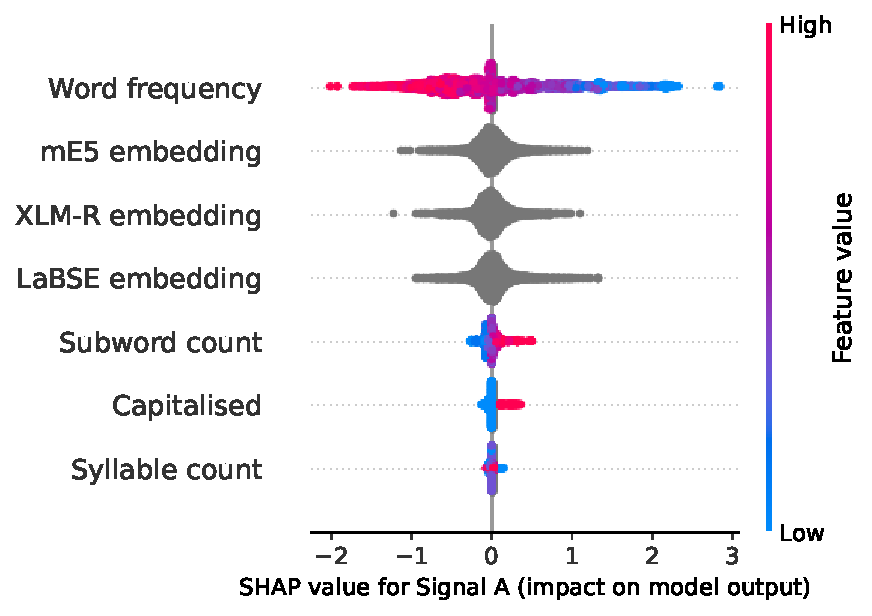
\includegraphics[width=\columnwidth]{fig_shap_signal_a_all.pdf}
\caption{SHAP values of all inputs of signal~A for the 7{,}211 instances, measured from the mean of
each instance's language, in standard deviations of signal~A within that language. The 768 embedding dimensions of each encoder are summed into one row, in
grey, since an embedding has no single value to colour.}
\label{fig:shap-all}
\end{figure}

\end{document}
